% uWaterloo Thesis Template for LaTeX
% Last Updated Nov 4, 2016 by Stephen Carr, IST Client Services
% FOR ASSISTANCE, please send mail to rt-IST-CSmathsci@ist.uwaterloo.ca

% Effective October 2006, the University of Waterloo
% requires electronic thesis submission. See the uWaterloo thesis regulations at
% https://uwaterloo.ca/graduate-studies/thesis.

% DON'T FORGET TO ADD YOUR OWN NAME AND TITLE in the "hyperref" package
% configuration below. THIS INFORMATION GETS EMBEDDED IN THE PDF FINAL PDF DOCUMENT.
% You can view the information if you view Properties of the PDF document.

% Many faculties/departments also require one or more printed
% copies. This template attempts to satisfy both types of output.
% It is based on the standard "book" document class which provides all necessary
% sectioning structures and allows multi-part theses.

% DISCLAIMER
% To the best of our knowledge, this template satisfies the current uWaterloo requirements.
% However, it is your responsibility to assure that you have met all
% requirements of the University and your particular department.
% Many thanks for the feedback from many graduates that assisted the development of this template.

% -----------------------------------------------------------------------

% By default, output is produced that is geared toward generating a PDF
% version optimized for viewing on an electronic display, including
% hyperlinks within the PDF.

% E.g. to process a thesis called "mythesis.tex" based on this template, run:

% pdflatex mythesis	-- first pass of the pdflatex processor
% bibtex mythesis	-- generates bibliography from .bib data file(s)
% makeindex         -- should be run only if an index is used
% pdflatex mythesis	-- fixes numbering in cross-references, bibliographic references, glossaries, index, etc.
% pdflatex mythesis	-- fixes numbering in cross-references, bibliographic references, glossaries, index, etc.

% If you use the recommended LaTeX editor, Texmaker, you would open the mythesis.tex
% file, then click the PDFLaTeX button. Then run BibTeX (under the Tools menu).
% Then click the PDFLaTeX button two more times. If you have an index as well,
% you'll need to run MakeIndex from the Tools menu as well, before running pdflatex
% the last two times.

% N.B. The "pdftex" program allows graphics in the following formats to be
% included with the "\includegraphics" command: PNG, PDF, JPEG, TIFF
% Tip 1: Generate your figures and photos in the size you want them to appear
% in your thesis, rather than scaling them with \includegraphics options.
% Tip 2: Any drawings you do should be in scalable vector graphic formats:
% SVG, PNG, WMF, EPS and then converted to PNG or PDF, so they are scalable in
% the final PDF as well.
% Tip 3: Photographs should be cropped and compressed so as not to be too large.

% To create a PDF output that is optimized for double-sided printing:
%
% 1) comment-out the \documentclass statement in the preamble below, and
% un-comment the second \documentclass line.
%
% 2) change the value assigned below to the boolean variable
% "PrintVersion" from "false" to "true".

% --------------------- Start of Document Preamble -----------------------


% Specify the document class, default style attributes, and page dimensions
% For hyperlinked PDF, suitable for viewing on a computer, use this:
\documentclass[letterpaper,12pt,titlepage,oneside,final]{book}

% For PDF, suitable for double-sided printing, change the PrintVersion variable below
% to "true" and use this \documentclass line instead of the one above:
%\documentclass[letterpaper,12pt,titlepage,openright,twoside,final]{book}

% Some LaTeX commands I define for my own nomenclature.
% If you have to, it's better to change nomenclature once here than in a
% million places throughout your thesis!
\newcommand{\package}[1]{\textbf{#1}} % package names in bold text
\newcommand{\cmmd}[1]{\textbackslash\texttt{#1}} % command name in tt font
\newcommand{\href}[1]{#1} % does nothing, but defines the command so the
    % print-optimized version will ignore \href tags (redefined by hyperref pkg).
%\newcommand{\texorpdfstring}[2]{#1} % does nothing, but defines the command
% Anything defined here may be redefined by packages added below...

% added by Yan
\usepackage{float}
\usepackage{tabularx}
\usepackage{svg}
\usepackage[ruled]{algorithm2e}
\usepackage{mdframed}
%--------This section has to do with todo notes ----------------
\usepackage{xargs}                      % Use more than one optional parameter in a new commands
\usepackage{etoolbox}
\usepackage[colorinlistoftodos,prependcaption]{todonotes}
\newcommandx{\intodo}[2][1=]{\todo[inline,#1]{#2}}
\newcommandx{\unsure}[2][1=]{\todo[linecolor=red,backgroundcolor=red!25,bordercolor=red,#1]{#2}}
\newcommandx{\change}[2][1=]{\todo[linecolor=blue,backgroundcolor=blue!25,bordercolor=blue,#1]{#2}}
\newcommandx{\info}[2][1=]{\todo[linecolor=OliveGreen,backgroundcolor=OliveGreen!25,bordercolor=OliveGreen,#1]{#2}}
\newcommandx{\improve}[2][1=]{\todo[linecolor=Plum,backgroundcolor=Plum!25,bordercolor=Plum,#1]{#2}}

\DeclareRobustCommand{\rintodo}[1]{%
  \todo[inline,linecolor=red,backgroundcolor=red!25,bordercolor=red]{#1}%
}

\addtocontents{toc}{\begingroup\protect\renewcommand{\protect\rintodo}[1]{}}
\AtEndDocument{%
  \addtocontents{toc}{\endgroup}
}

%----------------End of todo related stuff ----------------------




% This package allows if-then-else control structures.
\usepackage{ifthen}
\newboolean{PrintVersion}
\setboolean{PrintVersion}{false}
% CHANGE THIS VALUE TO "true" as necessary, to improve printed results for hard copies
% by overriding some options of the hyperref package below.

%\usepackage{nomencl} % For a nomenclature (optional; available from ctan.org)
\usepackage{amsmath,amssymb,amstext} % Lots of math symbols and environments
%\usepackage[pdftex]{graphicx} % For including graphics N.B. pdftex graphics driver


% Hyperlinks make it very easy to navigate an electronic document.
% In addition, this is where you should specify the thesis title
% and author as they appear in the properties of the PDF document.
% Use the "hyperref" package
% N.B. HYPERREF MUST BE THE LAST PACKAGE LOADED; ADD ADDITIONAL PKGS ABOVE
\usepackage[pdftex,pagebackref=false]{hyperref} % with basic options
		% N.B. pagebackref=true provides links back from the References to the body text. This can cause trouble for printing.
\hypersetup{
    plainpages=false,       % needed if Roman numbers in frontpages
    unicode=false,          % non-Latin characters in Acrobat’s bookmarks
    pdftoolbar=true,        % show Acrobat’s toolbar?
    pdfmenubar=true,        % show Acrobat’s menu?
    pdffitwindow=false,     % window fit to page when opened
    pdfstartview={FitH},    % fits the width of the page to the window
    pdftitle={uWaterloo\ LaTeX\ Thesis\ Template},    % title: CHANGE THIS TEXT!
%    pdfauthor={Author},    % author: CHANGE THIS TEXT! and uncomment this line
%    pdfsubject={Subject},  % subject: CHANGE THIS TEXT! and uncomment this line
%    pdfkeywords={keyword1} {key2} {key3}, % list of keywords, and uncomment this line if desired
    pdfnewwindow=true,      % links in new window
    colorlinks=true,        % false: boxed links; true: colored links
    linkcolor=blue,         % color of internal links
    citecolor=green,        % color of links to bibliography
    filecolor=magenta,      % color of file links
    urlcolor=cyan           % color of external links
}
\ifthenelse{\boolean{PrintVersion}}{   % for improved print quality, change some hyperref options
\hypersetup{	% override some previously defined hyperref options
%    colorlinks,%
    citecolor=black,%
    filecolor=black,%
    linkcolor=black,%
    urlcolor=black}
}{} % end of ifthenelse (no else)

\usepackage[automake,toc,abbreviations]{glossaries-extra} % Exception to the rule of hyperref being the last add-on package

% Setting up the page margins...
% uWaterloo thesis requirements specify a minimum of 1 inch (72pt) margin at the
% top, bottom, and outside page edges and a 1.125 in. (81pt) gutter
% margin (on binding side). While this is not an issue for electronic
% viewing, a PDF may be printed, and so we have the same page layout for
% both printed and electronic versions, we leave the gutter margin in.
% Set margins to minimum permitted by uWaterloo thesis regulations:
\setlength{\marginparwidth}{0pt} % width of margin notes
% N.B. If margin notes are used, you must adjust \textwidth, \marginparwidth
% and \marginparsep so that the space left between the margin notes and page
% edge is less than 15 mm (0.6 in.)
\setlength{\marginparsep}{0pt} % width of space between body text and margin notes
\setlength{\evensidemargin}{0.125in} % Adds 1/8 in. to binding side of all
% even-numbered pages when the "twoside" printing option is selected
\setlength{\oddsidemargin}{0.125in} % Adds 1/8 in. to the left of all pages
% when "oneside" printing is selected, and to the left of all odd-numbered
% pages when "twoside" printing is selected
\setlength{\textwidth}{6.375in} % assuming US letter paper (8.5 in. x 11 in.) and
% side margins as above
\raggedbottom

% The following statement specifies the amount of space between
% paragraphs. Other reasonable specifications are \bigskipamount and \smallskipamount.
\setlength{\parskip}{\medskipamount}

% The following statement controls the line spacing.  The default
% spacing corresponds to good typographic conventions and only slight
% changes (e.g., perhaps "1.2"), if any, should be made.
\renewcommand{\baselinestretch}{1} % this is the default line space setting

% By default, each chapter will start on a recto (right-hand side)
% page.  We also force each section of the front pages to start on
% a recto page by inserting \cleardoublepage commands.
% In many cases, this will require that the verso page be
% blank and, while it should be counted, a page number should not be
% printed.  The following statements ensure a page number is not
% printed on an otherwise blank verso page.
\let\origdoublepage\cleardoublepage
\newcommand{\clearemptydoublepage}{%
  \clearpage{\pagestyle{empty}\origdoublepage}}
\let\cleardoublepage\clearemptydoublepage

% Define Glossary terms (This is properly done here, in the preamble. Could be \input{} from a file...)
% Main glossary entries -- definitions of relevant terminology
\newglossaryentry{computer}
{
name=computer,
description={A programmable machine that receives input data,
               stores and manipulates the data, and provides
               formatted output}
}

% Nomenclature glossary entries -- New definitions, or unusual terminology
\newglossary*{nomenclature}{Nomenclature}
\newglossaryentry{dingledorf}
{
type=nomenclature,
name=dingledorf,
description={A person of supposed average intelligence who makes incredibly brainless misjudgments}
}

% List of Abbreviations (abbreviations type is built in to the glossaries-extra package)
\newabbreviation{aaaaz}{AAAAZ}{American Association of Amature Astronomers and Zoologists}

% List of Symbols
\newglossary*{symbols}{List of Symbols}
\newglossaryentry{rvec}
{
name={$\mathbf{v}$},
sort={label},
type=symbols,
description={Random vector: a location in n-dimensional Cartesian space, where each dimensional component is determined by a random process}
}

\makeglossaries

%======================================================================
%   L O G I C A L    D O C U M E N T -- the content of your thesis
%======================================================================
\begin{document}

% For a large document, it is a good idea to divide your thesis
% into several files, each one containing one chapter.
% To illustrate this idea, the "front pages" (i.e., title page,
% declaration, borrowers' page, abstract, acknowledgements,
% dedication, table of contents, list of tables, list of figures,
% nomenclature) are contained within the file "uw-ethesis-frontpgs.tex" which is
% included into the document by the following statement.
%----------------------------------------------------------------------
% FRONT MATERIAL
%----------------------------------------------------------------------
% T I T L E   P A G E
% -------------------
% Last updated Nov 1, 2016, by Stephen Carr, IST-Client Services
% The title page is counted as page `i' but we need to suppress the
% page number.  We also don't want any headers or footers.
\pagestyle{empty}
\pagenumbering{roman}

% The contents of the title page are specified in the "titlepage"
% environment.
\begin{titlepage}
        \begin{center}
        \vspace*{1.0cm}

        \Huge
        {\bf Efficient Structure-aware OLAP Query Processing over Large Property Graphs}

        \vspace*{1.0cm}

        \normalsize
        by \\

        \vspace*{1.0cm}

        \Large
        Yan Zhang \\

        \vspace*{3.0cm}

        \normalsize
        A thesis \\
        presented to the University of Waterloo \\ 
        in fulfillment of the \\
        thesis requirement for the degree of \\
        Master of Mathematics \\
        in \\
        Computer Science \\

        \vspace*{2.0cm}

        Waterloo, Ontario, Canada, 2017 \\

        \vspace*{1.0cm}

        \copyright\ Yan Zhang 2017 \\
        \end{center}
\end{titlepage}

% The rest of the front pages should contain no headers and be numbered using Roman numerals starting with `ii'
\pagestyle{plain}
\setcounter{page}{2}

\cleardoublepage % Ends the current page and causes all figures and tables that have so far appeared in the input to be printed.
% In a two-sided printing style, it also makes the next page a right-hand (odd-numbered) page, producing a blank page if necessary.
 


% D E C L A R A T I O N   P A G E
% -------------------------------
  % The following is a sample Delaration Page as provided by the GSO
  % December 13th, 2006.  It is designed for an electronic thesis.
  \noindent
I hereby declare that I am the sole author of this thesis. This is a true copy of the thesis, including any required final revisions, as accepted by my examiners.

  \bigskip
  
  \noindent
I understand that my thesis may be made electronically available to the public.

\cleardoublepage

% A B S T R A C T
% ---------------

\begin{center}\textbf{Abstract}\end{center}

Property graph model is a widely used model for real life systems of graph structure like social networks, financial transaction networks ect. On-Line Analytical Processing(OLAP) provides an important tool for data analyses by allowing users to perform data aggregation through different combinations of dimentions. For instance, with a Q\&A forum dataset, we may process queries like what is the average user's age group by post score to study if there is a correlation between age and post quality. With a music industry dataset, we may process queries like what is total sales of records group by music company and year to study market activities.

State-of-art graph databases like neo4j do not have efficient support for OLAP aggregation queries. For instance, Neo4j processes each OLAP query in two steps. First expand nodes and edges to the query structure, and then perform aggregation. Even if a query is repeatedly executed for multiple times, in each round Neo4j still processes the query from scratch, without gaining any "knowledge" from previous workload. When it comes to large property graphs, current graph databases' efficiency is far from satisfaction. It is unacceptable for users to wait for hours for results of a single query. 

We propose a system that greatly improves efficiency of OLAP over large property graphs. The idea is to smartly materialize some views(in main memory or hard disk) that a client was interested in based on a client's previous workload. Hopefully such materialization can be used to accelerate future query processing.  

We implemented our system on top of Neo4j and compared our system with orginal Neo4j system. We wrote some practical OLAP queries and randomly partition them into previous workload and future workload, and them executed future workload using both our system and Neo4j. Result shows that with an acceptable cost of memory or disk usage, we are able to improve OLAP processing efficiency by 10-30 times.  

\cleardoublepage

% A C K N O W L E D G E M E N T S
% -------------------------------

\begin{center}\textbf{Acknowledgements}\end{center}

I would like to thank Professor Tamer Ozsu and Dr. Xiaofei Zhang who made this thesis possible.
\cleardoublepage

% D E D I C A T I O N
% -------------------

\begin{center}\textbf{Dedication}\end{center}

This is dedicated to my mother Limei Leng whom I love.
\cleardoublepage

% T A B L E   O F   C O N T E N T S
% ---------------------------------
\renewcommand\contentsname{Table of Contents}
\tableofcontents
\cleardoublepage
\phantomsection    % allows hyperref to link to the correct page

% L I S T   O F   T A B L E S
% ---------------------------
\addcontentsline{toc}{chapter}{List of Tables}
\listoftables
\cleardoublepage
\phantomsection		% allows hyperref to link to the correct page

% L I S T   O F   F I G U R E S
% -----------------------------
\addcontentsline{toc}{chapter}{List of Figures}
\listoffigures
\cleardoublepage
\phantomsection		% allows hyperref to link to the correct page

% GLOSSARIES (Lists of definitions, abbreviations, symbols, etc. provided by the glossaries-extra package)
% -----------------------------
\printglossaries
\cleardoublepage
\phantomsection		% allows hyperref to link to the correct page

% Change page numbering back to Arabic numerals
\pagenumbering{arabic}



%----------------------------------------------------------------------
% MAIN BODY
%----------------------------------------------------------------------
% Because this is a short document, and to reduce the number of files
% needed for this template, the chapters are not separate
% documents as suggested above, but you get the idea. If they were
% separate documents, they would each start with the \chapter command, i.e,
% do not contain \documentclass or \begin{document} and \end{document} commands.
%======================================================================
\chapter{Introduction}
%======================================================================

%This thesis addresses that OLAP over large property graph is important but current graph databases process graph OLAP in an overwelmingly inefficient manner, and provides an end-to-end efficient solution for it.

Being a flexible and semantic rich model for graph structured data, the property graph model has been widely adopted and we have seen emerging Graph database systems supporting this model, like Neo4j \cite{DBLP:conf/oopsla/Webber12}, PGX \cite{DBLP:conf/sc/HongDMLVC15}. Supporting OLAP (On-Line Analytic Processing) is one critical feature of modern database systems, because efficient OLAP processing is fundamental to many decision-making applications, e.g., smart business~\cite{Petermann:2014:GDI:2733004.2733034,}, market analysis~\cite{DBLP:journals/corr/LamSG16,}, trend monitoring~\cite{DBLP:journals/tii/FangXZAPYL14,}, risk management~\cite{DBLP:journals/tcyb/ChoiCY17,}. However, empirical studies show that existing graph database systems do not efficiently support OLAP workloads, especially structure wise aggregation queries. Moreover, current graph database systems do not support view-based query or materialize some ``hot'' intermediate results to serve future queries. Therefore, in this thesis, we study the efficient processing of OLAP queries over property graph data using a materialization approach. 


%----------------------------------------------------------------------
\section{Property Graph Model}
%----------------------------------------------------------------------

We are living in an age with exponential growth of data, and a world that is more and more connected.  With the fast development of Web2.0 and Internet of Things(IoT)~\cite{DBLP:journals/cacm/X17f,}, numerous connections of various kinds are being created every second, producing massive amount of graph structure data in the meanwhile. For example, the moment a user creates a new post on a online forum, not only a post is created,  a ``\emph{creates}'' connection between the user and the post is established as well; when a user tags a post, a ``\emph{hasTag}'' connection is created between certain tag string and the post; or in a banking scenario, when a transfer happens, a ``\emph{transfers}'' connection between two accounts is created.

To capture the rich semantic of connected real-world entities, property graph model~\cite{} is becoming more and more popular considering its flexibility for semi-structured graph data. A property graph consists of nodes, edges, and properties. Like general graph data models, nodes represent entities and edges represent relationships. Graph nodes and edges can have any number of properties, or attributes, of any type. For example, Figure \ref{fig:1} shows a simple property graph of an online Q\&A forum named www.StackExchange.com. It shows the connections among users (represented by red nodes) and posts (represented by blue nodes). Each arc pointing from a user node  to a post node represents a ``User\_onws\_Post'' connection. From the graph, we can clearly see that  there is one user who has created one post while the other usr has created 2 posts. In addition, as shown in the example, a User node can have properties like the user’s Age, Views, UpVotes and etc. (listed at the end of the picture). 
%Notice that there is no restriction on what properties a User node can have. 
For clear presentation purpose, we shall use a property graph dataset obtained from \url{www.StackExchange.com} through this thesis. We name this graph ``StackExchange graph''. 


\begin{figure*}
\centering
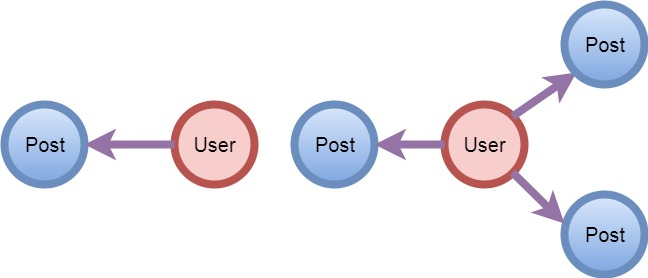
\includegraphics[scale=0.4]{pic/11.jpg}
\caption{A simple property graph modeling ``users post posts''(data graph).}
\label{fig:1}
\end{figure*}


%Besides nodes and edges, in property graph nodes and edges can have any number and type of properties. 


%For instance, in the exampling property graph,   That is, any node or edge could be freely attributed with any type of property. This makes a property graph very flexible in terms of property attribution.
 
%Property graph is an informative model as it contains not only nodes and edges, but properties of each individual node and edge as well. 

Note that although the property graph model does not enforce any restriction on what properties a node or edge can have, a highlevel abstraction describing the property relations, named the meta graph, is ofen defined in practice. Meta graph demonstrates the information of entities and entity correlations on a schema level, while data graph refers to the actual graph populated from the meta graph. Figure \ref{fig:2} and Figure \ref{fig:3} are the meta graph and a snapshot of the StackExchange graph, respectively. As shown in Figure \ref{fig:2}, there are three types of entities: User (in red), Post (in blue), and Tag (in green). Each user has a property named ``View'', each post has a property named ``Score'', and a property ``Tagname'' associated with each tag. There are two types of edges being  defined: User\_owns\_Post and Post\_hasTag\_Tag. 


\begin{figure*}[H]
\centering
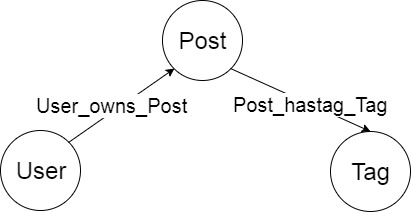
\includegraphics[scale=0.5]{pic/12.jpg}
\caption{Meta graph containing User, Post and Tag.}
\end{figure*}
 
\begin{figure*}[H]
\centering
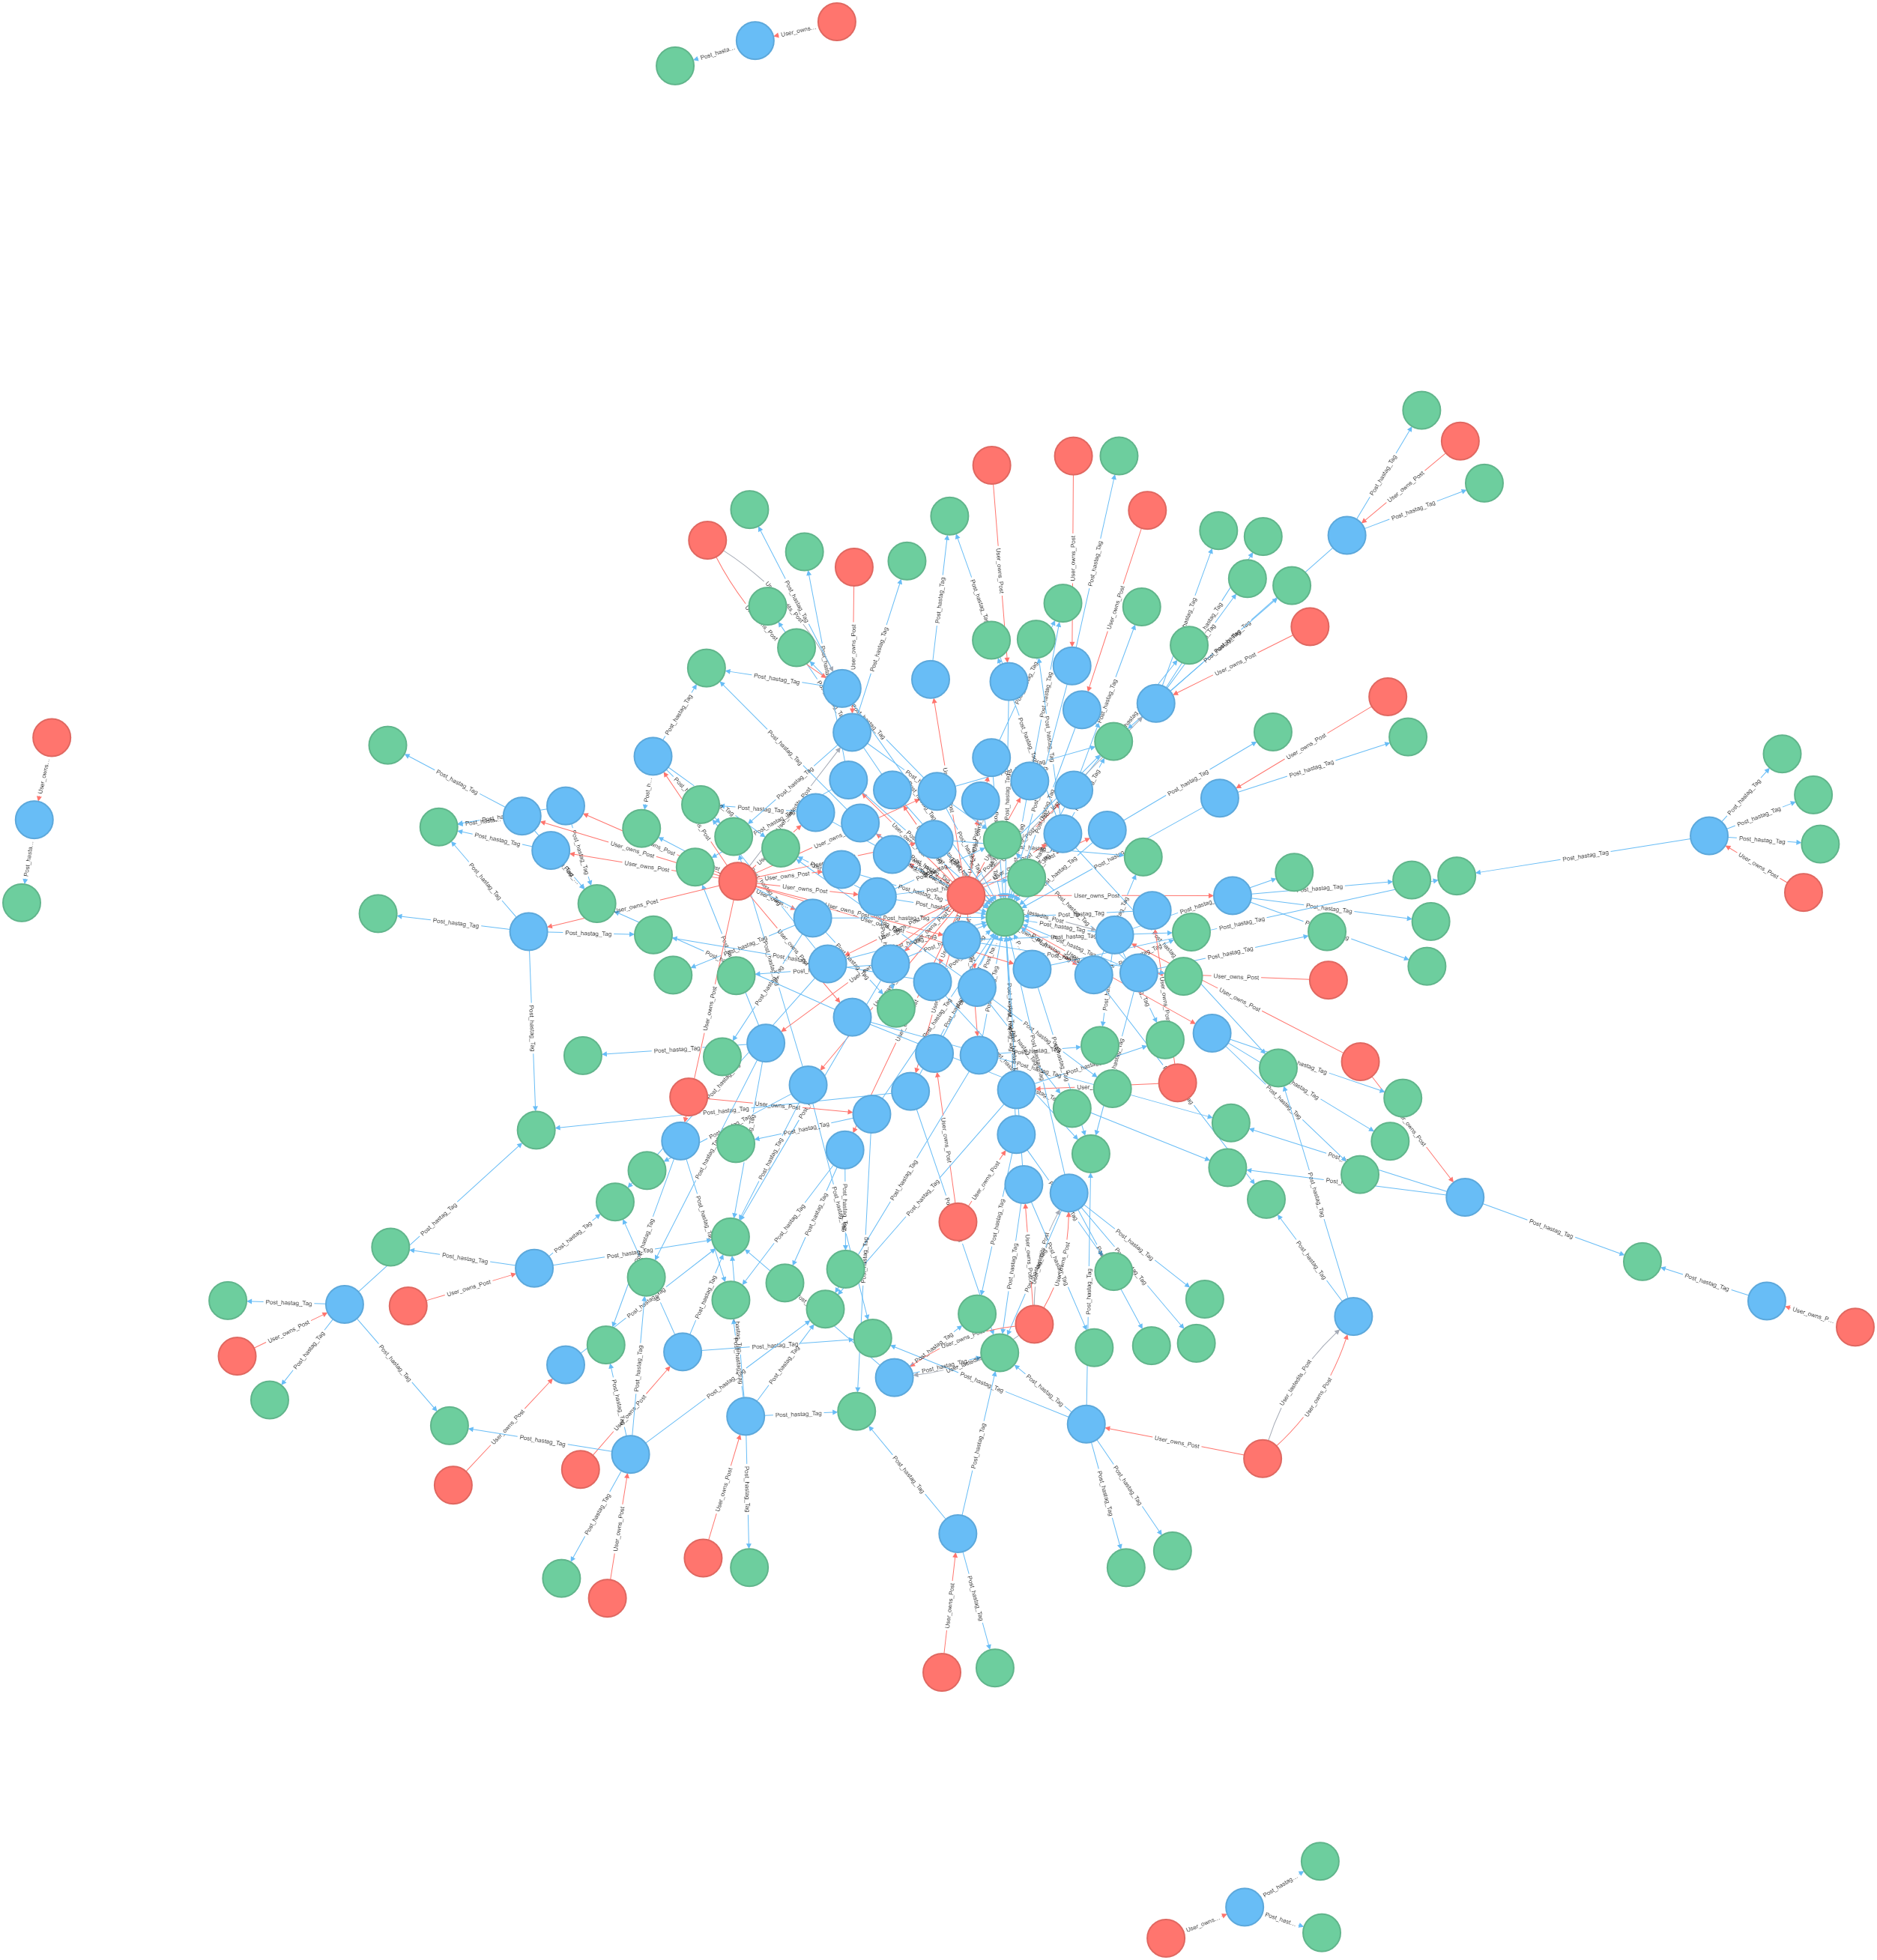
\includegraphics[scale=0.1]{pic/3.png}
\caption{A snapshot of data graph containing User, Post and Tag.}
\end{figure*}

%----------------------------------------------------------------------
\section{OLAP over Property Graph}
%----------------------------------------------------------------------
Among various kinds of queries, OLAP (Online analytical processing) queries play an important role in data analysis. 
\intodo{Add a few sentences to describe OLAP queries of the traditional database and warehousing applications. Showing it is important and we say performing OLAP on property graph is desired. }

In tradition databases and ware-housing, OLAP queries enable users to interactively perform aggregations on underlying data from different perspectives(combinations  of dimensions). There are three typical operations in OLAP. Roll-up operation allows user to view data in more details while drill-down operation does the opposite way. Slicing enables filtering on data. For instance, we can perform OLAP to analyze earning performance of an international company by different branch. We can perform drill-down operation by adding season as a dimension besides branch to take a closer look at profit performance of different branches in different seasons. In this case, OLAP serves as a tool for managers to better understand earning performance. 

Supporting efficient OLAP processing on property graphs grants users the power to perform insightful analysis over structured graph data. For example, on the StackExchange graph, users can study the correlation between the number of UpVotes and a post's score by using the following query:

\fbox{\emph{Get the average post score grouped by user’s upvotes.} }

 If the result shows a tight correlation, it suggests that an author’s upvotes can be used to estimate the quality of his or her post when a post is freshly posted and score of the post has not been settled.


Consider another example, using a property graph dataset on music industry,  one can issue the following query to evaluate a company's strategy to increase the share of young people's market.

\fbox{
\begin{minipage}{35em}
\emph{Get the total sum of music purchases by buyers at age 18-25 grouped by music company and month}
\end{minipage}
}


For simplicity, we call such kind of OLAP query workloads over property graphs as ``Graph OLAP''. As a matter of fact, graph OLAP has already been applied in various senerios like business analysis and decision making and it is attracting increasing research interests in the database community.



%----------------------------------------------------------------------
\section{Challenges of Graph OLAP}
%----------------------------------------------------------------------

%We know that Graph OLAP is important. However there are many challenges on this topic. One of the most challenging part is efficiency issue. 
\intodo{Here you should start with a paragraph saying "Supporing efficient OLAP is traditional RDBMS or warehousing applications is a well studied topic. There are abundent literature attacking this problem from virous different perspectives, e.g. data partition~\cite{}, view selection~\cite{}, partial materialization~\cite{}, .... However, there is very few research effort on the Graph OLAP. Existing literatures concerning OLAP workload over graph data either target on accelerating graph OLAP over a special subset of property graphs~\cite{}, or focus on generic highlevel topics, such as ... \cite{},  other than time efficiency issue of query processing."}

Supporting efficient OLAP in traditional RDBMS or warehousing applications is a well studied topic. There are abundent literature attacking this problem from virous different perspectives, e.g. data partition~\cite{DBLP:conf/ismis/CuzzocreaL12,}, view selection~\cite{DBLP:books/igi/Taniar10/LawrenceR10,}, partial materialization~\cite{DBLP:journals/kais/DrzadzewskiT16,}, .... However, there is very few research effort on the Graph OLAP. Existing literatures concerning OLAP workload over graph data either target on accelerating graph OLAP over a special subset of property graphs~\cite{DBLP:conf/sigmod/ZhaoLXH11}, or focus on generic highlevel topics, such as \cite{DBLP:conf/esws/MaaliCD15} \cite{DBLP:conf/icdm/ChenYZHY08},  other than time efficiency issue of query processing.

%From an academic point of view, most of OLAP studies reside in traditional relational data models, whereas studies on efficient graph OLAP are not enough. What's worse, current graph OLAP researches either  

Our empirical studis show that existing graph databases do not provide efficent support for graph OLAP, especially when the graph size scales to real-word practices, which usually contains over millions of nodes and edges. %Graph databases are databases that specialize in storage and processing of property graphs. However current graph databases are not satisfactory in terms of OLAP processing efficiency over large property graphs(often with more than millions of nodes and edges). 
To elaborate, Neo4j, a state-of-art graph database, processes OLAP queries in a rather straightforward manner: computing everything from scratch for each query without being aware of any history workloads. In an extreme case, even if we executed the same query repeatly with only minor change on value constraints, e.g., change the constraint of user's age from 20 to 22, the execution plan always stays the same and yields no execution time improvement.  

\begin{figure*}[H]
\centering
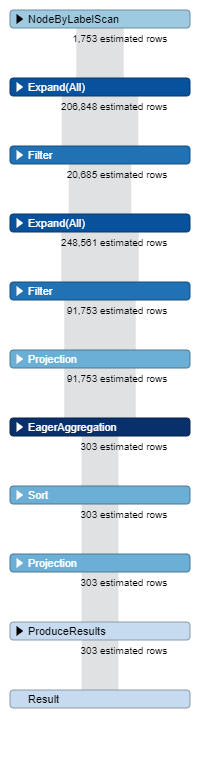
\includegraphics[scale=0.4]{pic/5.png}
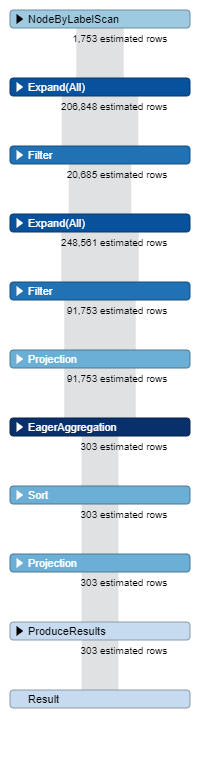
\includegraphics[scale=0.4]{pic/5.png}
\caption{Execution plans of Query \#3 for first time and fifth time.}

\end{figure*}

%This naive feature of always executing queries regardless of previous queries misses valuable information contained in previous workloads.
Valuable information extracted from history workload can be helpful to accelerate in-coming query processing. For example, the above exampling OLAP query on StackExchange graph dataset (of roughly 45GB in size) takes Neo4j more than 2 hours to process. It is frustrating for users to wait that long for the result of one single OLAP query, as it undermines interactivity which is one of the most distinctive features of OLAP. %Therefore we want to accelerate OLAP processing over large property graphs
\intodo{Now you should explain what you can learn from previous workloads, and how these knowledge can help you with future workloads.}

As a matter of fact, history workloads provide useful information for future workloads. This is because in real case users do not generate OLAP queries randomly. Instead users often tend to be interested in some specific ``hot'' structures on a meta graph level and some ``hot'' properties. Such interest is contained in history workload and can serve as an insightful hint on future workloads. Suppose we sacrifice some memory space and materialize ``hot'' structures and properties even before future queries arrive, future queries can be faster processed.  

\intodo{Then, you need a paragraph that describe the actual challenge. Because so far you only mentioned that using something from history workload is helpful, then the problem is how to extract these information, how to decide which information should be materialized espeically when there is a space constraint.}

We know that materialization on user's interested structures and properties results in benefit on future workload processing efficiency , and cost on memory space. The real challenge is how to design a score function to evaluate the trade-off  between such benefit and cost so that we can use the score function to select best materialization. Here best materialization refers to the case where we achieve best future workload acceleration with a given memory constraint for materialization.

%\begin{center}
%	\begin{tabular}{ | l | l | } 
%		\hline 
%		Query 	& Time	\\ \hline 
%		Query \#1	& \\ \hline
%		Query \#2	& \\ \hline
%		Query \#3	& \\ \hline
%	\end{tabular}
%	\end {center}
	
	


%----------------------------------------------------------------------
\section{Our Solution and Contributions}
%----------------------------------------------------------------------
To address the challenges discussed above, we propose a end-to-end solution for graph database to  support efficient  OLAP over large property graphs.

The essence of our solution is to precompute and materialize popular intermediate results that can be reused by future workloads. Intuitively, in real practice, most OLAP queries from the same client   tend to reside in several particular structures and properties (usually closely related with the topics that the client is interested in). Within a specific period of time, there are ``hot'' structures that the client tends to repeatedly investigate from different dimensions. Therefore, previous queries can be used as a good reference to discover structures and properties in which the client is particularly interested. 

%For instance, suppose a client just executed the exampling four queries, here is what we can learn from these four previous workload:

%Structure-wise: (User)-[creates]-$>$(Post) is frequently queried. We can tell that client is interested in how users create posts. Thus it is reasonable to guess that the user is likely to issue OLAP queries involving (User)-[creates]-$>$(Post) in following queries.
 
%Property-wise: User.UpVotes, Post.Score, User.Age, Tag.TagName etc. More specifically, \{User.UpVotes, Post.Score\} and \{User.Age, Tag.TagName\} are frequent combinations. Thus it makes sense to guess that these property combinations are likely to appear together in future queries.
 
%Intuitively, if we smartly select frequently queried structures and properties based on previous workload and materialize them, they might be covered in future queries and thus be used to accelerate processing. 
 
A good analogy of this is establishment of materialized views in relational databases and processing queries directly on materialized views. In relational databases, we are allowed to build materialized views on structures and attributes that we are interested in. Hopefully when future queries come, we can faster process them using pre-materialized views. Unfortunately, current graph databases do not support similar operations. 
 
%Therefore we propose a system that realizes automatic and smart pre-computing and materialization based on history workload, and utilize the materialized result to accelerate future query processing. 
 
There are two most important problems that we need to solve: 
 
One key issue is smart selection of ``materialized views''. We need to select and pre-compute those that are most beneficial for future queries. 
 
Another key issue is how to optimize a better execution plan for answering a future query efficiently using the precomputed materials.

\intodo{here you need to use a paragraph to explain how you select materialized views, e.g., you develop a cost function. Plus, you have a scheduling policy to execute subqueries in the most time efficient way. This part is particularly important, because reader need to briefly understand you overall solution from a high level perspective.}

For the first issue, we develop a score function to evaluate cost–performance ratio of a materialization. We propose a greedy  algorithm to  select candidate  based on their score(calculated from score function), one by one until memory limit is hit.

For the second issue, if a future query result can be directly produced using a materialization we simply do it. For other cases, we propose a scheduling policy to decompose a future query into substructures and join such substructures to produce final result.  

To highlight, we summurize our contributions in this thesis as follows:
\begin{itemize}
\item {We designed an end-to-end system that realizes structure-aware OLAP query processing on graph databases using precomputation based on previous workloads.}

\item We implemented our system on Neo4j.

\item We proposed our algorithm for smart selection of structures and cuboids to be precomputed.
 
\item We suggested different ways for future query processing. We tested their performances and gave explanations on the performance differences.
 
 \end{itemize}

The following contents are organized as follows:
 we discuss the preliminaries and related work in Chapter 2. Followed by the background knowledge about  OLAP, graph databases, and Neo4j, we give a summarization of existing literatures concerning OLAP queries over graph data. In Chapter 3 we explain our solution framework and system design in details. We present the experiment design and result disucssion in Chapter 4. Chapter 5 concludes this thesis with highlight on opening questions and future work.




%======================================================================
\chapter{Background and Related Work}
%======================================================================
In this chapter, we first explain graph OLAP with real examples. Then we briefly introduce Neo4j, a state-of-art graph database system, which is employed as the back end of our proposed solution. In addition, we review and summarize the most recent relevant works on graph OLAP processing.


%----------------------------------------------------------------------
\section{OLAP over Property Graph Model}
%----------------------------------------------------------------------


Following the introduction of the property graph model given in the previous chapter, we further define the syntax of properties adopted in this thesis. In the property graph model, each node and edge could have arbitrary number and type of properties. A type of property is represented as follows:

\begin{displaymath}
\centering
[NodeType].[PropertyType]
\end{displaymath}

For example, User.Age denotes an ``Age'' attribute associated with a node of type ``User''. In order to identify a node or edge, a unique ID is assigned to each node and edge.  For simplicity, in this thesis we represent a node or an edge with its ID, denoted as ID(node) or ID(edge). Note that unique ID is sometimes treated as a special type of property.


OLAP (On-Line Analytical Processing) \cite{DBLP:conf/sigmod/BeyerR99, DBLP:journals/datamine/GrayCBLRVPP97, DBLP:conf/sigmod/ZhaoDN97} usually employs a cube concept, which is constructed over multiple attributes, in order to provide users a multi-dimensional and multi-level view for effective data analysis from different perspectives and with multiple granularities. The key operations in an OLAP framework are slice/dice and roll-up/drill-down, with slice/dice focusing on a particular aspect of the data, roll-up performing generalization if users only want to see a concise overview, and drill-down performing specialization if more details are needed. We shall detail the cube technique from the graph data perspective later this chapter.

 Graph OLAP is first proposed by Graph Cube \cite{DBLP:conf/sigmod/ZhaoLXH11}. It refers to OLAP over graphs. Though no formal definition of the notion ``Graph OLAP'' is given in \cite{DBLP:conf/sigmod/ZhaoLXH11}. Graph Cube \cite{DBLP:conf/sigmod/ZhaoLXH11} views the outcome of Graph OLAP as aggregated graphs (aggregation of data graph). On the contrary, in our work, we consider the outcome of Graph OLAP as result tables of OLAP queries.

 Graph Cube \cite{DBLP:conf/sigmod/ZhaoLXH11}  addresses and defines two most important notions in graph OLAP scenarios as \textit{dimension} and \textit{measure}. In our work emphasize \textit{structure} (of meta graph) as a third important notion. Graph Cube \cite{DBLP:conf/sigmod/ZhaoLXH11} focuses more on OLAP senerios over a fixed \textit{structure}, with \textit{dimension} and \textit{measure} varied. %Therefore, there is no need to emphasize and discover the notion of \textit{structure}. 
 In our work, we are able to deal with OLAP workloads over various \textit{structures}.

 %The ``graph'' in our work refers to property graphs. As introduced in Section 1.1, property graph is more flexible and powerful than classic attribute graphs.

\subsection{OLAP Examples}
\label{OLAPExamples}
 In order to better elaborate how ``Graph OLAP'' is interpreted in our thesis, consider the following four example scenarios, where we perform OLAP queries over the StackExchange graph.

\noindent\textbf{Example 1} Does the number of high upvotes of a user indicate a high-quality post?

\fbox{
Query \#1: Get average post score grouped by user’s upvotes.
}

Sample query result:
\begin {center}
\begin{tabular}{ l l }
	User.UpVotes&AVG(Post.Score)\\\hline
	0&1.33\\
	1&2.23\\
	2&2.34\\
	3&2.77\\
	4&3.43\\\hline
\end{tabular}
\end {center}

From the query result we can see that upvotes can be used as a good indicator of a user’s post quality. Suppose we would like to propose suggested posts based on scores. When a post is freshly posted and score of the post has not been well voted been yet, we may use the author’s upvotes as a factor to estimate the quality of his or her post.

\noindent\textbf{Example 2} Following the context of Query \#1, but this time we want to take a closer look at Query \#1 for different types of questions. If we take upvotes as quality of a user, perhaps quality of a user is shown only in his or her answers, instead of questions. Or is it true that high quality user also asks much better questions?

\fbox{
Query \#2:  Get average post score grouped by user’s upvotes and post’s post types.
}

Sample query result:

\begin {center}
\begin{tabular}{ l l l }
	User.Upvotes&Post.PostTypeId&AVG(Post.Score)\\\hline
	0&1&2.14\\
	1&1&2.26\\
	2&1&2.83\\
	3&1&3.04\\
	4&1&3.46\\
	0&2&1.54\\
	1&2&2.21\\
	2&2&2.18\\
	3&2&2.72\\
	4&2&3.58\\\hline
\end{tabular}
\end {center}

The query results suggest that high-quality users not only provide good answers but ask valuable questions as well. However, there is a subtle difference on how upvotes is correlated with questions and answers. For example, a really low upvote level indicates a low-quality answer more than a low-quality question. This is probably because people tend to be more tolerate with a naive question rather than a wrong answer.

Query \#1 and Query \#2 simply focus on relationship between User and Post. We may switch our attention to a slightly more complicated structure by adding the Tag.

\noindent\textbf{Example 3} In year 2017, which is the weighted average age of users? For instance is ‘python’ more trendy than ‘c’ among young users?

\fbox{
Query \#3: Get average user age grouped by users’ 2017 posts’ tags.
}

Sample query result:

\begin {center}
\begin{tabular}{ l l  }
	
	TagName&AVG(Age)\\\hline
	Router&19.6\\
	Python&24.1\\
	Internet&26.8\\
	C&30.2\\
	programmer&31.4\\
	software&29.8\\\hline
	
\end{tabular}
\end {center}

From the results, one can tell the average user age with respect to each tag clearly and easily compare them. It reveals some interesting insight: python is generally more popular among younger users; and  ``Router'' is a relatively ``younger'' topic than ``Internet''.

\noindent\textbf{Example 4} Find out the tendency of topic’s ``average popular user age'' by years. Is there a tendency of younger age?

\fbox{
Query \#4: Get average user age grouped by users’ posts’ tags and years.
}

Sample query result:

\begin {center}
\begin{tabular}{ l l  l}
	
	TagName & Year & AVG(Age) \\\hline
	Router & 2012 & 22.1 \\
	Router & 2017 & 19.6 \\
	Python & 2012 & 27.3 \\
	Python & 2017 & 24.1 \\
	Internet & 2012 & 27.5 \\
	Internet & 2017 & 26.8 \\
	C & 2012 & 30.4 \\
	C & 2017 & 30.2 \\
	programmer	& 2012 & 34.2 \\
	programmer	& 2017 & 31.4 \\
	software	& 2012 & 31.6 \\ 
	software	& 2017 & 29.8\\\hline
	
\end{tabular}
\end {center}

Tendency of younger age on IT topics is revealed from the results. Python is getting faster embraced by younger people compared with C. Similarly we can compare two commercial products’ customer targeting strategy, advertising performance etc.

From the above OLAP query examples we can see that OLAP over property graphs provides an interactive and informative way to analyze property graphs from multiple dimensions, and thus helps people find the hidden correlations, aggregated effects, regularities, tendencies and so on.

\subsection{Structure, Dimension, and Measure}

We now explain the three key elements of a graph OLAP: \textit{structure}, \textit{dimension}, and \textit{measure}  using Query \#1 as an example.

%\textbf{Query \#1: 		Get average post score grouped by user’s upvotes. }

Query \#1 is concerns the following structure (colored in blue) on the meta graph:

\begin{figure}[H]
\centering
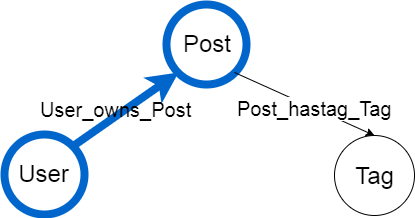
\includegraphics[scale=0.5]{pic/meta1.png}
\caption{\textit{Structure} of Query \#1}
\label{fig:2:1}
\end{figure}



We say that (User)-[User\_owns\_post]-$>$(Post) is the structure of Query \#1. The query is first aggregated on user’s upvotes. We say that {User.Upvotes} is the dimension of Query \#1. And the output of the query is an aggregation function on post’s score.  We say that {AVG(Post.Score)} is the measure of Query \#1. Similarly, consider the above Example 2, which shares the same structure as shown in Figure \ref{fig:2:1}. The dimensions of Query \#2 is {User.Upvotes, Post.PostTypeId}, and the measure is {AVG(Post.Score)}. Note that Query \#2 adds Post.PostTypeId to Query \#1’s dimensions. In other words, Query \#2 asks for a more detailed partitions over dimensions. We call Query \#2 a drill-down from Query \#1, and  Query \#1 is a roll-up from Query \#2. Note that possible property combinations can be modeled as a lattice-structured cube. Figure \ref{fig:2:2} shows what a cube is like for properties \{A,B,C\}. We can see that roll-up and drill-down operations allow us to navigate up and down on a cube.


\begin{figure}[H]
\centering
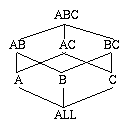
\includegraphics[scale=1]{pic/22.png}
\caption{Cube of properties \{A,B,C\}.}
\label{fig:2:2}
\end{figure}

\textbf{Query \#3: 		Get average user age grouped by users’ 2017 posts’ tags.}

Structure:	(User)-[User\_owns\_post]-(Post)-[Post\_hastag\_Tag]-(Tag)
\begin{figure}[H]
\centering
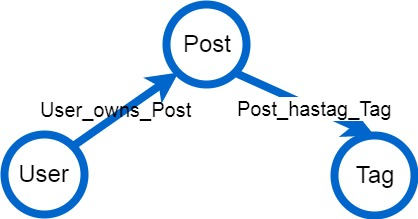
\includegraphics[scale=0.5]{pic/meta2.jpg}
\caption{\textit{Structure} of Query \#3}
\label{fig:2:3}
\end{figure}


Dimensions:	{Tag.Tagname}

Measures:	{AVG(User.Age)}

Note that Query \#3 has a different \textit{strucutre} than Query \#1 and Query \#2, as shown in Figure \ref{fig:2:3}. Query \#3 enforces a requirement that post must be created in year 2017, which picks out a particular subset of  the posts. In OLAP this is called ``slicing'' operation. Slicing operation allows users to view the data with filtering requirements on selected properties. In this thesis we call the constraint {Post.Year=2017}  of Query \#3 a \textit{``slicing condition''}.

To summarize, graph OLAP allows clients to aggregate different \textit{structures}, over different \textit{dimensions}, on different \textit{measures}, and optionally slice aggregation result by different \textit{slicing conditions}. Clients can change their views by performing roll-up, drill-down, and slicing freely and interactively.


%----------------------------------------------------------------------
\section{Graph Databases and Neo4j}
%----------------------------------------------------------------------
 Emerging online applications concerning graph processing has motivated the relational database community to support efficient graph management~\cite{}. However, there has been active debate about the efficiency of using traditional RDBMS for graph computing considering the unique query workload against graph data~\cite{}, which is beyond the scope of this thesis. As a matter of fact, relational databases and graph databases both have their own strengths in term of query processing.  It is generally accepted that graph databases perform better at property graph data processing as it conforms more with the actual graph structure. For clear presentation purpose, we highlight some key differences between the RDBMS and graph database. 

%There are two major types of databases that store and process graph data: traditional relational databases and graph databases.

Relational databases  model graph data as entity and relationship tables. For example, given a simple property graph shown in Figure \ref{fig:2:4}, which consists of 1 user and 3 posts, a relational database stores the graph with 3 tables:

\begin{figure}[H]
\centering
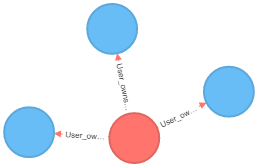
\includegraphics[scale=0.9]{pic/4.png}
\caption{A simple property graph.}
\label{fig:2:4}
\end{figure}


\begin{center}
\begin{tabular}{|c|c|c| }
	\hline
	\multicolumn{3}{|c|}{User} \\\hline
	Uid	& Age & UpVote	\\ \hline
	1 & 22 & 5 \\\hline
\end{tabular}
\end {center}


\begin{center}
	\begin{tabular}{|c|c|}
	\hline
	\multicolumn{2}{|c|}{Post} \\\hline
		Pid	& Score	\\ \hline
		1	& 0.5 \\
		2	& 0.8 \\
		3	& 0.6 \\\hline
	\end{tabular}
	\end {center}	


\begin{center}
	\begin{tabular}{|c|c|}
	\hline
	\multicolumn{2}{|c|}{Owns} \\\hline
		Uid	& Pid	\\ \hline
		1	&1 \\
		1	&2 \\
		1	&3 \\\hline
	\end{tabular}
	\end {center}


There are two drawbacks of storing property graphs in a relational database. First, each node or edge in a property graph could have arbitrary types of properties. However, relational table schema would restrict nodes or edges of the same type to have a uniform set of properties (attributes). Second and more importantly, edges are stored as a separate table in relational databases. Thus, we cannot directly query all the posts of a given user without joining User and Own tables in the above example.

Graph databases solve the above two issues by directly adopting property graph structures to store data. In graph databases, edges are stored not as independent tables but directly attached to related nodes using data structures such as adjacency lists. Many graph database applications have been implemented and commercialized. One of the popular ones is Neo4j, which holds atomicity, consistency, isolation, durability (ACID) as traditional RDBMS does. Database instances in Neo4j are modeled and stored as  property graphs. %Like other graph databases, edges are not stored as physically separate tables, but directly attached to their nodes. 
One thing special about Noe4j’s property graph is that its nodes and edges can be labeled with any number of labels (similar to entity and relationship types). For example, a node referring to a student could have various labels such as “student”, “people” etc.

Cypher is Neo4j’s query language, which is expressive and simple. For example, consider the following query: what is the average score group by different user upvotes when PostTypeID is 2? A Cypher query would be written as follows:

\begin{verbatim}
match (u:User)-[r:User\_owns\_Post]-$>$(p:Post) 
where p.PostTypeId=`2' 
return u.Upvotes, AVG(p.Score)
\end{verbatim}

In the above Cypher query, ``User'' and ``Post'' are node labels, PostTypeId and Score are properties of ``Post'', ``UpVotes'' is a property of ``User''.

%Neo4j is written in Java. While applications in various languages could interact the server by issuing queries and transport using BOLT protocol. BOLT protocol is a binary protocol implemented by Neo4j team. It is more efficient than HTTP protocol.

%Figure 2.4 shows how applications interact with Neo4j server.
%
%\begin {figure}[H]
%\centering
%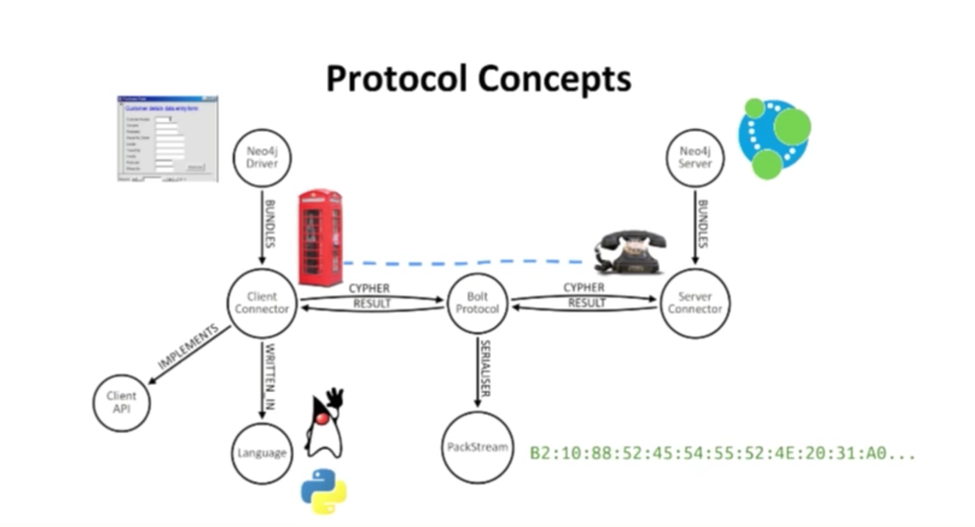
\includegraphics[scale=0.4]{pic/23.png}
%\caption{How applications interact with Neo4j server.}
%\end{figure}


%----------------------------------------------------------------------
\section{Related Work}
%----------------------------------------------------------------------

There have been a few work discussing efficient graph OLAP queries on attribute graphs or RDF graphs. 

Cube-based \cite{DBLP:conf/sofsem/JakawatFL16} proposes the concept of  graphs enriched by cubes. Each node and edge of the considered network are described by a cube. It allows the user to quickly analyze the information summarized into cubes. It works well in slowly changing dimension problem in OLAP analysis. 

Gagg \cite{DBLP:conf/esws/MaaliCD15} introduces an RDF graph aggregation operator that is both expressive and flexible. It provides a formal definition of Gagg on top of SPARQL Algebra and defines its operational semantics and describe an algorithm to answer graph aggregation queries. Gagg achieves significant improvements in performance compared to plain-SPARQL graph aggregation.

Pagrol \cite{DBLP:conf/icde/WangFWTAA14} provides an efficient MapReduce-based parallel graph cubing algorithm, MRGraph-Cubing, to compute the graph cube for an attributed graph.

%Graph Cube \cite{DBLP:conf/sigmod/ZhaoLXH11} introduces Graph Cube, a new data warehousing model that supports OLAP queries effectively on large multidimensional networks. It takes account of both attribute aggregation and structure summarization of the networks. In order to deal with “curse of dimensions”, a greedy algorithm framework is introduced for partial materialization of cuboids. 

Graph OLAP \cite{DBLP:conf/icdm/ChenYZHY08} studies dimensions and measures in the graph OLAP scenario and furthermore develops a conceptual framework for data cubes on graphs. It differentiates different types of measures(distributive and holistic etc) by their properties during aggregation. It looks into different semantics of OLAP operations, and classifies the framework into two major subcases: informational OLAP and topological OLAP. It points out a graph cube can be fully or partially materialized by calculating a special kind of measure called aggregated graph.

In Graph Cube \cite{DBLP:conf/sigmod/ZhaoLXH11}, concepts of graph cube is introduced. Given a particular structure S, a property set P, and measure set M. We can aggregate over S on $2^{|P|}$ different combinations of dimensions. These $2^{|P|}$ queries can be mapped as a lattice structure, where each combination of dimensions corresponds to a cuboid in the lattice. We call the lattice structure of these $2^{|P|}$ queries a graph cube.


It has been pointed out in  Graph OLAP \cite{DBLP:conf/icdm/ChenYZHY08} that as long as if domain of measure is within \{count, sum, average\} and M contains count(*), the following feature holds: given any two cuboids $C_1$ and $C_2$ from the same graph cube, as long as dimension($C_2$) is a subset of dimension($C_1$), result of $C_1$ can be used to generate result of $C_2$. This is to say once a cuboid is materialized, all roll-up operations from this cuboid could be processed simply by scanning the materialized cuboid result. This will dramatically decrease roll-up operation time compared to aggregation from data graph(often of larger size, disk I/O), scanning materialized cuboid result(often of smaller size) is often much faster.


Ideally we can materialize all cuboids. But when number of dimension is large, number of cuboids grows exponentially, making total materialization impossible due to overwhelming space cost. To solve this Graph Cube \cite{DBLP:conf/sigmod/ZhaoLXH11} proposed a partial materialization algorithm on graph cube. It is a greedy algorithm and the score function is based on benefits of deduction of total computation cost.

We summarize some of the most related ones as follows:
 \begin{table}
 	\footnotesize
 \begin{center}
 	\begin{tabular}{ | c | c | c | c | c |  }
 		\hline
 		 & G. Type & Q. Pattern & Layered & Featuer\\ \hline
 		 Cube-based \cite{DBLP:conf/sofsem/JakawatFL16} & Property & Simple relation & yes & Cubes on edges and nodes\\ \hline
 		 Gagg \cite{DBLP:conf/esws/MaaliCD15} & Property & Exact match & no & Structural patterns\\ \hline
 		 Pagrol \cite{DBLP:conf/icde/WangFWTAA14} & Property & edge \& node attributes & yes & Map-Reduce computing\\ \hline
 		 Graph Cube \cite{DBLP:conf/sigmod/ZhaoLXH11} & Homogenous  & node attributes & yes & Partial materialization\\ \hline
 		 Graph OLAP \cite{DBLP:conf/icdm/ChenYZHY08} & Property & edge \& node attributes & yes & Distributive and holistic measures\\ \hline
 		
 	\end{tabular}
 	\end {center}
 	\caption{A summary of graph OLAP literature}
\end{table}


From the summary, we can categorize the existing work into two lines. First, like Graph Cube \cite{DBLP:conf/sigmod/ZhaoLXH11}, researches focus on a simple subset of property graphs(e.g. graphs with only homogenous nodes and edges) and proposes optimizations in order to accelerate OLAP query processing. The optimizations are attribute-aware, and since the nodes and edges are of only one kind queries over different structures and structure-aware optimizations are out of the scope. Second, like Gagg \cite{DBLP:conf/esws/MaaliCD15}, researches focus on an abstract high-level framework that process generic queries over generic property graphs. However, query processing efficiency is not studied.

To conclude, we can see a lack of study on structure-aware optimizations for efficient graph OLAP. As mentioned in Section 1.3, efficiency issue is one of the most challenging issues on graph OLAP. Therefore, it is very meaningful to explore faster structure-aware OLAP processing over general property graphs.



%----------------------------------------------------------------------
%\section{Graph Cube}
%----------------------------------------------------------------------





%======================================================================
\chapter{Problem Definition}
%======================================================================
In this section, we first illustrate the terminology and notations adopted in this work. Then we formally define the problem of efficient OLAP query processing. 

%----------------------------------------------------------------------
\section{Terminologies}
%----------------------------------------------------------------------

This section gives definations and notations of property graph, queries, materializations. Besides, we introduce concepts of ``cuboid'' and ``subsubstrcutre'', which are two types of materializaitons we will use in our solution. 

\subsection{Defination of Property Graph}
We define a property graph as $G(V, Vid, E, Eid, A, L, f)$ where  $V$ is a set of nodes. $Vid$ is set of unique IDs of $V$. $E$ is a set of edges. $E \subseteq V * V$. $Eid$ is set of unique IDs of $E$. $A$ is a set of properties. $L$ is a set of labels. $f$ is mapping function that maps $V$ and $E$ to $A$, $L$, $Vid$ and $Eid$: $f_{VA}: \{V_{i} \rightarrow A_{i}\}, V_{i}\in V, A_{i} \subseteq A$ , maps each node to its properties; $f_{VL}: \{V_{i} \rightarrow L_{i}\}, V_{i}\in V, L_{i} \subseteq L$ , maps each node to its labels; $f_{EA}: \{E_{i} \rightarrow A_{i}\}, E_{i}\in E, L_{i} \subseteq A$ , maps each edge to its properties; $f_{EA}: \{E_{i} \rightarrow L_{i}\}, E_{i}\in E, L_{i} \subseteq L$ , maps each edge to its labels; $f_{VID}: \{V_{i} \rightarrow Vid_{i}\}, V_{i}\in V, Vid_{i} \subseteq N$ , maps each node to its unique ID; $f_{EID}: \{E_{i} \rightarrow Eid_{i}\}, V_{i}\in V, Eid_{i} \subseteq N$ , maps each edge to its unique ID.

%\begin{itemize} 
%\item $V$ is a set of nodes. $Vid$ is set of unique IDs of $V$.
%\item $E$ is a set of edges. $E \subseteq V * V$. $Eid$ is set of unique IDs of $E$.
%\item $A$ is a set of properties.
%\item $L$ is a set of labels.
%\item $f$ is mapping function that maps $V$ and $E$ to $A$, $L$, $Vid$ and $Eid$. 
%
%$f_{VA}: \{V_{i} \rightarrow A_{i}\}, V_{i}\in V, A_{i} \subseteq A$ , maps each node to its properties.
%
%$f_{VL}: \{V_{i} \rightarrow L_{i}\}, V_{i}\in V, L_{i} \subseteq L$ , maps each node to its labels.
%
%$f_{EA}: \{E_{i} \rightarrow A_{i}\}, E_{i}\in E, L_{i} \subseteq A$ , maps each edge to its properties.
%
%$f_{EA}: \{E_{i} \rightarrow L_{i}\}, E_{i}\in E, L_{i} \subseteq L$ , maps each edge to its labels.
%
%$f_{VID}: \{V_{i} \rightarrow Vid_{i}\}, V_{i}\in V, Vid_{i} \subseteq N$ , maps each node to its unique ID.
%
%$f_{EID}: \{E_{i} \rightarrow Eid_{i}\}, V_{i}\in V, Eid_{i} \subseteq N$ , maps each edge to its unique ID.
%
%\end{itemize} 

\subsection{Notations on OLAP Query}

As discussed before, Four elements of a graph OLAP query are \textit{Structure}, \textit{Dimension}, \textit{Measure}, and \textit{Slicing Condition}(optional). We will introduce how we represent these four elements and an OLAP query. We will use Query \#3 in Chapter 2 as an example.

\textbf{\textit{Structure:}} A \textit{strucuture} consists of \textit{edges}. We write a \textit{structure} by listing all its \textit{edges} seperated by comma, where an \textit{edge} is represented by 

\fbox{
	\textit{Starting Node Label- Edge Label- Ending Node Label} 
}

For instance, Query \#3's \textit{structure} as shown in \ref{fig:2:3} is written as 

\textit{``User-owns-Post, Post-has-Tag''}



\textbf{\textit{Dimension:}} A
\textit{Dimension} is written by listing all properties that act as dimensions in an OLAP query.

Query \#3's \textit{dimension} is written as

\textit{``Tag.Tagname''}

\textbf{\textit{Measure:}} We focus on three most common types of \textit{measure}: \textit{COUNT(*), SUM and AVG. }

Query \#3's \textit{measure} is written as

\textit{``AVG(User.Age)''}


\textbf{\textit{Slicing Conditions:}} A \textit{Slicing Conditions} is written as 

\fbox{
$Property = value$
}

Query \#3's \textit{slicing conditions} is written as

\textit{``Post.Year=2017''}

\textbf{\textit{OLAP query:}} With the four elements ready, we write an entire OLAP query as 

\fbox{
	\textbf{\textit{Structure : Dimension, Measure, Slicing Condition}}
}

Query \#3 is written as 

fbox{
\textit{User-owns-Post, Post-has-Tag: Tag.Tagname, AVG(User.Age), Post.Year=2017
}

where \textit{User-owns-Post, Post-has-Tag} referring to  \textit{structure}, \textit{Tag.Tagname} referring to \textit{dimension},\textit{ AVG(User.Age) } referring to \textit{measure}, {Post.Year=2017} referring to \textit{slicing condition}. Note that since \textit{dimension}, \textit{measure} and \textit{slicing condition} are written in different forms, it is easy to distinguish them even if they are all listed together.


 \textbf{\textit{Features of a query:}} For a query q, we use ``q.properties'' to refer to a set of \textbf{all properties} in \textit{Dimension, Measure, and Slicing Condition} of q. We use ``q.structure'' to refer to structure of q.

 \textit{Query \#3.properties=\{Tag.Tagname, User.Age, Post.Year\}}
 
 \textit{Query \#3.structure= User-owns-Post, Post-has-Tag}



\subsection{Materialization: Cuboid vs Substructures}
\label{Materialization: Cuboid vs Substructures}

We want to accerlerate OLAP by materializations from previous workload. We use

\fbox{
	\textbf{\textit{\$Query}} 
}

to refer to materializaiton of a $Query$.

As we mentioned before, in a property graph each node and edge has a unique ID, which can be treated as a special property. Whether a materialization keeps unique ID is an important issue, as keeping unique ID often increases space cost of a materialization. We categorize two types of materializaitons, ``cuboid'' and ``substructure'', based on whether unique IDs of nodes and(or) edges are kept or not. To better understand ``cuboid'' and ``substructure'', let's look at the following example.


Suppose we have following previous workload and future workload:

Previous workload \#1 User-owns-Post: User.Age\\
Previous workload \#2 User-owns-Post: User.Age, (AVG)Post.Score\\
Future workload \#1 User-owns-Post: (AVG)User.Age, Post.Score	\\
Future workload \#2 User-owns-Post, Post-has-Tag: User.Age, Tag.TagName




%User-owns-Post: User.Age
%
%User-owns-Post: User.Age, (AVG)Post.Score
%
%User-owns-Post, Post-has-Tag: User.Age, Tag.TagName

We can tell that the user is most interested in  \textit{User-owns-Post} structure. \{User.Age, Post.Score\} is the set of properties that are involved in queries over \textit{User-owns-Post} . We can build a cuboid lattice of all combinations of  \{User.Age, Post.Score\}. Materialization of base cuboid of the lattice is

\fbox{
\textit{\$User-owns-Post: User.Age, Post.Score, COUNT(*)}
}

\textit{\$User-owns-Post: User.Age, Post.Score, COUNT(*)} is useful for future workload \#1. We can process future workload \#1 by aggregation over \textit{\$User-owns-Post: User.Age, Post.Score, COUNT(*)}. We call such materilization a \textbf{``cuboid''}.


However, \textit{\$User-owns-Post: User.Age, Post.Score, COUNT(*)} is not useful for future workload \#2. The reason is that they have different \textit{structures}.


If we add ID(Post) into \textit{dimension} and materialize \textit{\$User-owns-Post: User.Age, Post.Score, ID(Post) COUNT(*)}, \textit{Post} is ``activated'' to be able to join with other materializations containing \textit{Post} and produce results for OLAP over more complicated \textit{structures}. For instance, future workload \#2 can be processed by 


1.joining \textit{\$User-owns-Post: User.Age, Post.Score, ID(Post) COUNT(*)} and \textit{\$Post-has-Tag: ID(Post), Tag.TagName, COUNT(*)} on ID(Post)

2.aggregation on \{User.Age, Tag.TagName\}. 

In this case, we only need to fetch \textit{\$Post-has-Tag: ID(Post), Tag.TagName, COUNT(*)} from database to produce result for future workload \#2. We call such materialization with ID(s) in \textit{dimension} \textbf{``substructure''}. 

Note that cuboids can only be used in queries with exactly the same structure. They can be be scanned for more aggregated dimension combinations(drill-down operations) but they are not useful for queries with different \textit{structures}. 

Substructures can be used to join with other materializations to help with future queries of various types of \textit{structures}.
The drawback is that structures are generally more space-costly than cuboids, as IDs are unique keys. The trade-off between cuboids and substructures is \textbf{\textit{space vs joining potential}}.

\ref{Table:3:1} gives a summary of comparisions between ``cuboid'' and ``substructure''. 

 \begin{table}
	\footnotesize
\begin {center}
\begin{tabular}{ | l | l | l |}
	\hline
 &Cuboid&Substructure\\ \hline
 Dimension& Only properties& Properties and ID(s)\\ \hline
 Space Cost& ``Low''&``High''\\ \hline
 Potential benefit& Aggregation& Aggregation \& Joining\\ \hline
\end{tabular}
\end {center}
\caption{Comparisons between Cuboid and Substructure.}
\label{Table:3:1}
\end{table}


%----------------------------------------------------------------------
\section{Problem Definition}
\label{sec:Problem Definition}
%----------------------------------------------------------------------

Our target is to faster process future OLAP workload using materializations computed based on previous workload. We can divide our goal in two steps. 
\begin{itemize}
	\item Materializaiton Step: clever selection of views for materialization. 
	\item Query Processing Step: processing future queries in shortest time(using materializaitons). 
\end{itemize} 

Materializaiton Step requires us to solve ``Materialization Selection Problem''. Query Processing Step requires us to solve ``Processing Plan Problem''. We give definations for these two problems as follows.

\textbf{``Materialization Selection Problem'':}

Using materialization is good for query efficiency, but comes with a storage cost. So we want to study the problem of how to best utilize materialization within a space budget limit $\sigma$. 


\\
We define ``Materialization Selection Problem'' as

Given a property graph dataset G, a set of previous queires P on G, space limit $\sigma$, find cuboids C and substructures S, $\displaystyle{\sum_{c_{i}\in C}c_{i}.estimatedSpace} + 
\displaystyle{\sum_{s_{i}\in S}s_{i}.estimatedSpace} 
\leq \sigma
$, so that 

$\displaystyle{\sum_{p_{i}\in P}estimatedProcessingTime(G, p_{i}, C, S)}$  is minimized.

Here $estimatedProcessingTime(p_{i}, C, S)}$ is a function for estimation of query processing time of $p_{i}$ on G using materializations of C and S, and ``estimatedSpace'' refers to estimation of space cost of a cuboid or substructure. Note that we need estimation of time and space cost because it is hard to know the exact actual costs without actually running queries.

%Is ``Processing Plan Problem'' even considered as a problem?
 
\textbf{``Processing Plan Problem'':}

We define ``Processing Plan Problem'' as


Given a property graph dataset G, a future query q, materialized cuboids C and substructures S, find a processing plan $process(G, q, C, S)$, so that $process(G, q, C, S).executionTime$ is minimized. 

We further divide ``Processing Plan Problem'' into two sub-problems. ``View Decomposition Problem'' decompose q into views from C and S (which have been materialized) and remaining views (which will be fetched from database server). ``View Operation Problem'' performs basic table operations such as joining, projection, selection over views in order to generate result of q.

``View Decomposition Problem'':
Given a property graph dataset G, a future query q, materialized cuboids C and substructures S, select $C' \subseteq C, S'\subseteq S$, and $R$  a processing plan $process(G, q, C, S)$, so that $process(G, q, C, S).executionTime$ is minimized.
 


%======================================================================
\chapter{Solution}
%======================================================================





%----------------------------------------------------------------------
\section{Solution Framework}
%----------------------------------------------------------------------

Our solution framework (Figure \ref{Solution framework}) contains two major parts. ``Materialization Part'' takes previous workload as input and perform materialization. We first partition previous queries into ``hot'' queries and ``less hot'' queries based on frequency count of their structures. CubePlanner and StructurePlanner take ``hot'' queries and ``less hot'' queries as input and select cuboids and substructures (in form of tables) for materialization respectively. Subsection \ref{Overview of Materialization Part} will explain intuition of categorization of ``hot'' and ``less hot'' queries and why we pass them to different ``planners''.  ``Future Query Processing Part'' takes future queries as input and generate results. If a future query is of ``hot'' structure we consult cuboid materializations to see if it can be directly answered by aggregation over a cuboid materialization. In this scenario cuboid materialization will be used. If the future query cannot be directly answered by any cuboid materialization, we turn to substructure materializations. We decompose the query into substructures and produce results by ``joining'' these substructures. In this scenario, substructure materializations will be used. 

We will discuss ``Materialization Part'' in Section \ref{Materialization Part} and ``Future Query Processing Part'' in Section \ref{Future Query Processing Part}.

\begin {figure}[H]
\centering
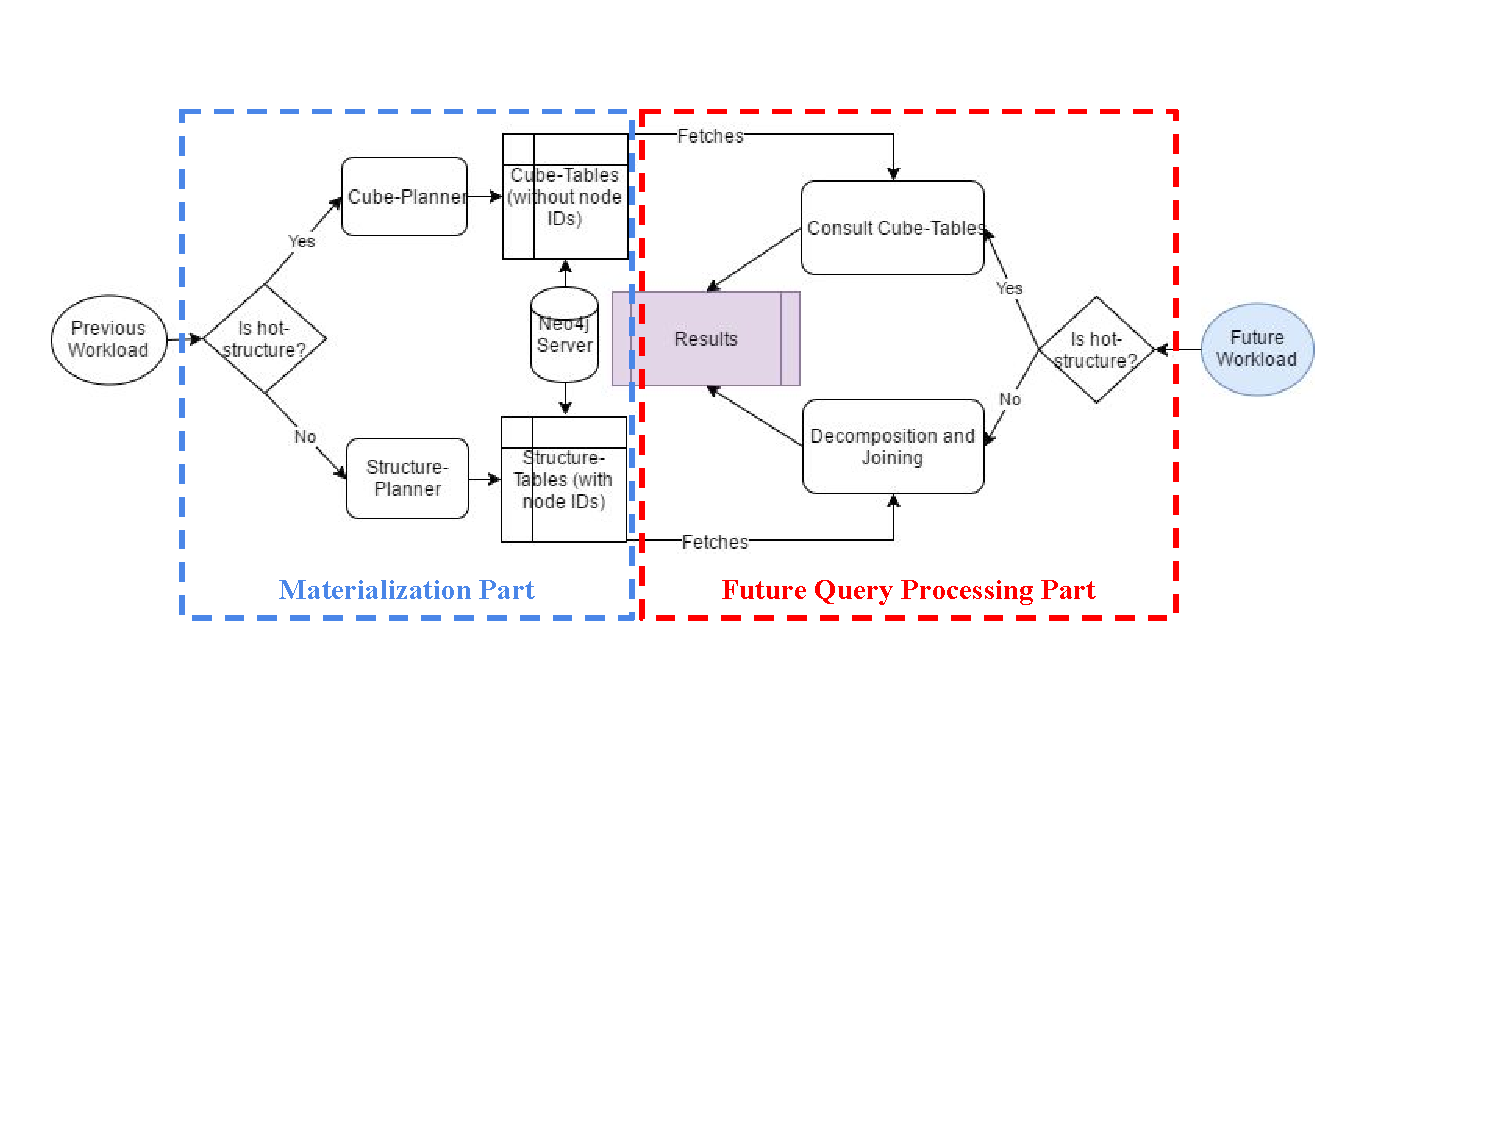
\includegraphics[scale=0.8]{pic/41.pdf}
\caption{Solution framework.}
\label{Solution framework}
\end{figure}


%----------------------------------------------------------------------
\section{Materialized View Selection}
\label{Materialization Part}
%----------------------------------------------------------------------
We will discuss materialized view selection in this section. We will first give an overview of materialized view selection and then focus on cuboid and substructure selections respectively.
%----------------------------------------------------------------------
\subsection{Overview of Materialized View Selection}
\label{Overview of Materialization Part}
%----------------------------------------------------------------------
In Section \ref{Materialization: Cuboid vs Substructures}, we have discussed about the trade-off between cuboids and substructures. We know that utilization of a cuboid materialization requires future queries to have exactly the same structure as the cuboid. It is wise that we materialize a cuboid only when we are confident that the structure of a cuboid is likely to be ``hit'' by future queries, because otherwise we may risk wasting space only to materialize cuboids that are rarely ``hit''. Compared with cuboids, substructures do not have such strict ``structure match'' requirement. A substructure can be used as long as it is covered by a future query. 

We make our materialization policy based on such different features of cuboids and substructures. 
We first perform frequency count of previous queries. For queries of structure frequency over a threshold $\sigma$, consider these queries have ``hot structure'' and pass them to CubePlanner for cuboid selection. For the rest queries with "less hot structure", pass them to StructurePlanner for substructure selection. 

\begin{algorithm}[H]
\caption{Materialization Overview}
\LinesNumbered
\textbf{System setting:} $\sigma$: frequency threshold for hot structures\\ 
\KwIn{Q: a set of previous queries\\}
\KwOut{C: a set of materialized cuboids\\ S: a set of materialized substructures}

$CInput \gets \emptyset$\;
$SInput \gets \emptyset$\;
\ForEach{q \in Q}{
	\eIf{structureFreq(Q, q) $>$ \sigma}{
		$CInput \gets CInput \cup \{q\} $\;
	}{	
		$SInput \gets SInput \cup \{q\} $\;
	}
}
$C:=materialize(CubePlanner(CInput))$\;
$S:=materialize(StructurePlanner(SInput))$\;
\label{alg:PartialMaterialization}
\end{algorithm}
\clearpage

Function $structureFreq(Q, q)$ returns frequency count of $q$'s structure in $Q$. Functions $CubePlanner$ and $StructurePlanner$  return selected cuboids and substructures by CubePlanner and StructurePlanner. Function $materialize$ performs materialization of cuboids and substructures.

For example, suppose we have the following previous queries and future queries.

\textbf{Previous Workload:}

\begin{itemize}
\item \#1 Badge-User, User-Post:Badge.Name,Post.Score,Post.PostTypeId=2

\item \#2 User-Comment, Comment-Post: User.UpVotes, Comment.Score, (AVG)Post.Score, Post.PostTypeId=1

\item \#3 User-Post, Post-Vote: User.UpVotes, Vote.VoteTypeId

\item \#4 User-Post, Post-Tag: (AVG)User.CreationDate\_Year, Tag.TagName

\item \#5 User-Comment, Comment-Post: User.ActiveMonth, Post.CreationDate\_Year=2016

\item \#6 User-Comment, Comment-Post: User.Age, (AVG)Comment.Score, Post.PostTypeId=2
\end{itemize}


\\
\textbf{Future Workload:}

\begin{itemize}
\item \#1 User-Comment, Comment-Post: User.UpVotes, (AVG)Post.Score, Post.PostTypeId

\item \#2 User-Comment, Comment-Post: User.Age, Post.PostTypeId

\item \#3 User-Post, Post-PostHistory: User.UpVotes, PostHistory.PostHistoryTypeId

\item \#4 Badge-User, User-Post:(AVG)Post.Score,Post.PostTypeId=2
\end{itemize}

\par
We count previous queries by structure:

\begin{center}
\begin{tabular}{ | c | c |}  
	\hline
	Structure	&Frequency	\\ \hline 
	\textbf{User-Comment, Comment-Post} 	&\textbf{3} \\ \hline
	User-Post, Post-Tag 	&1 \\ \hline
	User-Post, Post-Vote	&1 \\ \hline
\end{tabular}
\end {center}
\par	
We are confident that \textit{User-Comment, Comment-Post} is a ``hot structure''. We materialize cuboids over structure \textit{User-Comment, Comment-Post} by passing previous query \#2, \#5 and \#6 to CubePlanner. CubePlanner will materialize cuboids that benefit processing of future query \#1 and \#2 (which have \textit{User-Comment, Comment-Post} structure).
\par
We pass the three remaining queries of ``less hot structure'' previous query \#1, \#3 and \#4 to StructurePlanner. StructurePlanner will discover and materialize most useful substructures. In this case StructurePlanner is likely to find \textit{User-Post} as a useful substructure it can be used in joining the result of future query \#3 and \#4.
%----------------------------------------------------------------------
\subsection{Greedy Selection Framework}
%----------------------------------------------------------------------

We adopt a greedy selection framework in materialized view selection. In our solution framework, CubePlanner and StructurePlanner are responsible for materialized view selection (over cuboids and substructures respectively). They both adopt the same greedy selection framework. In Section \ref{sec:Problem Definition}, we introduced that ``Materialization Selection Problem'' aims at finding best materializations under a space limit $\sigma$. ``Materialization Selection Problem'' is known to be an NP-hard problem \cite{DBLP:journals/kais/LinK04}. It is hard because overall benefit of materialized views is not a simple sum of individual benefit of each materialized view. A materialized view's marginal benefit may be deducted when another view is selected. For example, marginal benefit of a substructure over ``\textit{User-Post, Post-Tag}'' will be affected by selection of substructures over ``\textit{User-Post}'' and ``\textit{Post-Tag}''. A naive approach to solve ``Materialization Selection Problem'' is to enumerate over all possible combinations of cuboids $C$ and substructures $S$ within the space limit $\sigma$ and find the best combination. But such naive may results in an unacceptable time complexity. What's worse, suppose we find an answer $C'$ and $S'$ in a naive way. It is not guaranteed that actual total space cost of $C'$ and $S'$ is strictly lower than $\sigma$ as we made estimations in our calculation. As a result, we turn to a greedy algorithm which is better than naive approach in terms of efficiency, besides it allows materializations to be done one by one until space limit $\sigma$ is hit.

We will discuss this greedy selection framework first so that readers have a high-level idea of our selection policy. We use greedy algorithms for cuboid and substructure selection. The idea is to always pick next candidate with highest ratio of margin benefit against space. After a candidate is picked, we re-evaluate benefit of remaining candidates. Re-evaluation is essential as margin benefit of a candidate may be deducted owing to materialization of a selected candidate. 


\begin{algorithm}[H]
	\caption{Greedy Selection}
	\LinesNumbered  
	\textbf{System setting:} $\sigma$: space limit\\ 
	\KwIn{C: a set of candidates of cuboids or substructures in lattice structure\\ P: A set of previous queries}
	\KwOut{Q: a queue of selected candidates to materialize\\ }
	\ForEach{c \in C}{
		c.space := space(c)\;
		c.benefit := estimateMarginBenefit(c, P, Q)\;
		c.score := c.benefit/c.space\;
	} 
	
	\While{$Q.totalsize < \sigma$}{
		selected := c in C with highest score\;  
		Q.Enqueue(selected)\;
		repeat Lines 1-5\;
	}
\end{algorithm}

We use a queue as data structure for output $Q$ in above algorithm presentation because in some cases we may want to keep information of orders of selection. When selection orders are not important we may as well simply use a set to store selected views. Line 1-5 estimates space cost, marginal benefit for future workload, and score for each candidate. We call this parse  \textbf{``score calculation''}. Line 6-10 keeps picking up candidates with highest score one by one until space limit is hit. Notice that each time a candidate is selected, Line 9 refreshes scores for all candidates by repeating 1-5. We call this parse \textbf{``pick-and-update''}.   

CubePlanner and StructurePlanner apply this greedy selection framework by implementation of ``score calculation'' and ``pick-and-update''. Future users can vary CubePlanner and StructurePlanner by plug-ins of their own implementation with consideration of their database features. We will introduce how we implement our CubePlanner and StructurePlanner for Neo4j in the following subsections.

%----------------------------------------------------------------------
\subsection{CubePlanner}
%----------------------------------------------------------------------  

We will discuss CubePlanner in this subsection. CubePlanner takes ``hot'' previous queries as input and output selected cuboid materializations. In Subsection \ref{Materialization: Cuboid vs Substructures}, we mentioned that one feature about cuboid is that cuboid are only useful for queries of exactly same structure. To put it another way, cuboids of different structures do not affect each other at all in terms of benefits for future queries. As a result even though input queries for CubePlanner may have different structures, we can group queries by structure and treat them individually. For each group of input queries we propose algorithm ``SingleCubePlanner'' to select top-$n$ cuboids. After all groups are finished, we select final results across top-$n$ cuboids of all groups. A good analogy for such process is to first hold regional competitions and then select national winners from regional winners. Next we will explain ``CubePlanner'' and ``SingleCubePlanner'' in details.

%----------------------------------------------------------------------
\subsubsection{CubePlanner}
\label{CubePlanner}
%---------------------------------------------------------------------- 

As we mentioned above, CubePlanner performs cuboid selection in a holistic manner by one-by-one selection of cuboids from results of SingleCubePlanners. 

\begin{algorithm}[H]
	\caption{CubePlanner}
	\LinesNumbered 
	\textbf{System setting:} 
	: maximum number of cuboids to precompute\\ 
	\KwIn{Q: a set of previous queries not nessesarily with a same structure}
	\KwOut{C: a queue of selected cuboids to precompute\\ }
	Group:= group(Q)\;
	\ForEach{group \in Group}{
		group.results := SingleCubePlanner(group);
	} 
	
	\For{i=1 \emph{\KwTo} n}{
		group' := group in Group with highest group.results.top().score\; 
		C.offer(group'.Dequeue())\;
	}
	
\end{algorithm}
\clearpage

Function $group(Q)$ groups $Q$ by structure. $SingleCubePlanner$ will be discussed in Subsection \ref{SingleCubePlanner}. 

Line 1 partitions $Q$ by structure. Each partition consists of previous queries of a same structure, which will be passed to a SingleCubePlanner. Line 2-4 performs cuboid selection in each partition using SingleCubePlanner. An ordered queue of candidates is generated by each SingleCubePlanner. Line 5-8 repeatedly checks current top candidate for each partition and picks out the best candidate among them. $n$ is a user defined parameter. In our implementation select $n$ at most cuboids for materialization.  Users may choose other ways such as a space limit as a bound for cuboid materiliazation.

%----------------------------------------------------------------------
\subsubsection{SingleCubePlanner}
\label{SingleCubePlanner}
%----------------------------------------------------------------------  

Given previous queries of a same structure, we implement algorithm ``SingleCubePlanner'' from greedy selection framework to select top-$n$ cuboids. 

\begin{algorithm}[H]
	\caption{SingleCubePlanner}
	\LinesNumbered 
	\textbf{System setting:} n: as in ``top-$n$''\\ 
	\KwIn{P: a set of previous queries with a same structure}
	\KwOut{C: an queue of selected cuboids to precompute\\ }
	$Lattice \leftarrow buildLattice(Q)$\;
	\ForEach{query $Q$ \in P}{
		$q.time \leftarrow time(q)$\;
	} 
	\ForEach{cuboid \in Lattice}{
		$cuboid.space \leftarrow space(cuboid) $\;
		$cuboid.benefit \leftarrow 0$\;
		\ForEach{query $Q$ $\in$ $P$ and q.properties $\subseteq$ cuboid.properties}{
			$cuboid.benefit +=max(0, q.time-aggreTime(cuboid))$\;
		}
		$cuboid.score \leftarrow cuboid.benefit/cuboid.space$\;
	}
	\For{i=1 \emph{\KwTo} n}{
		nextBestCube $\gets$ cuboid in Lattice with highest score\;
		\If{$nextBestCube.score < 0$}{
			break\;
		}
		C.Enqueue(nextBestCube)\;
		\ForEach{cuboid $Q$ $\in$ $Q$ and q.dimension $\subseteq$ nextBestCube.dimension }{
			$q.time \gets min(q.time, aggreTime(nextBestCube)) $\;
		}
		repeat 5-12\;
	}
	
\end{algorithm}
\clearpage

Line 1 builds a lattice over all combinations of dimensions of all attributes which appeared in previous queries $P$ using classic lattice construction algorithms \cite{DBLP:journals/ipl/NourineR99}. Line 2-4 initializes best-so-far processing time for each previous query by its estimated naive database processing time. Line 5-12 performs ``score calculation'' in ``greedy selection framework''. For each cuboid, Line 6 estimates its space. Line 8-10 calculates marginal benefit. Line 8 iterates over previous queries that can be answered by scanning current cuboid. If estimated scanning time is less than a previous query's current best-so-far processing time, we add the difference of two times to the cuboid's total marginal benefit (Line 9). Line 13-23 performs ``pick-and-update'' in ``greedy selection framework''. Line 15-17 terminates selection when there is no extra marginal benefit any more. Line 19-22 updates best-so-far processing time for previous queries as a result of current round of selection.

Implementation of functions are listed as follows. Notice that users can implement these functions in their own ways based on their database systems. Function \textbf{$time(query)$} estimates naive time cost for processing a query by a graph database. Implementation of $time(query)$ is database specific as physical storage and execution plans vary among different databases. Since Neo4j provide APIs to see execution plan and estimated intermediate result size, we directly use total size of intermediate results as an estimation of time cost. For example, Figure \ref{fig:4:2} is an execution plan provided by Neo4j for query \textit{User-Badge, User-Post, Post-Tag: Tag.TagName}. We can see that numbers of ``estimated rows'' for intermediate results are provided. We use  $\displaystyle{\sum ``estimated\_rows''}$ to estimate total processing time cost.

\begin {figure}[H]
\centering
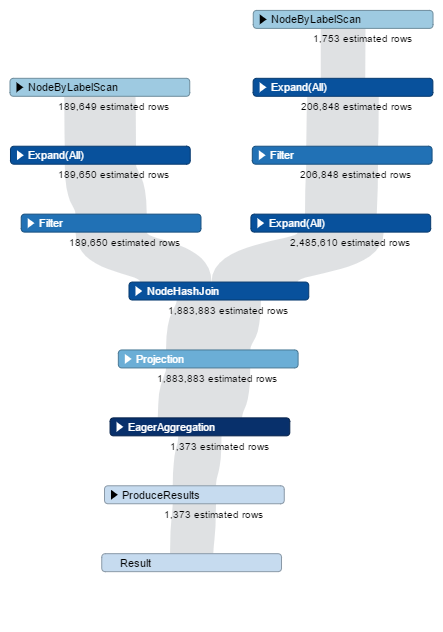
\includegraphics[scale=0.6]{pic/61.png}
\caption{Neo4j's execution plan for query \textit{User-Badge, User-Post, Post-Tag: Tag.TagName}.}
\label{fig:4:2}
\end{figure}

For graph databases where such APIs to see  execution plans and estimated intermediate result sizes are not provided, users need to provide estimation based on their understanding about the database. There are many studies on cost estimations for database operations (joins etc). Users may consider joining (expanding) order \cite{DBLP:conf/pods/Chaudhuri98} and estimation of intermediate result sizes  \cite{DBLP:conf/edbt/SwamiS94} as two important aspects. 

Function \textbf{$aggreTime(cuboid)$} estimates time cost for a scanning cuboid materialization. For cuboid $c$, we use space cost of $c$ for estimation. 

$spacePerRow:= 
\displaystyle{\sum_{p\in c.properties}sizeOf(p)}$

$SpaceCost(c):= spacePerRow *  numberOfRows(c)$

Here \textit{sizeOf(property type)} refers to standard size of data types. For exmaple integer type in ``C++'' is 2 byte. \textit{numberOfRows(c)} refers to number of rows of $c$. A rough estimation is the product of cardinalities of all queried properties. 

$numberOfRows(c):= \displaystyle{\prod_{p\in c.properties}|p|} $


%----------------------------------------------------------------------
\subsection{Structure Planner}
\label{Structure Planner}
%----------------------------------------------------------------------
Like CubePlanner, Structure Planner also adopts greedy selection framework.

\begin{algorithm}[H]
\caption{StructurePlanner}
\LinesNumbered 
\textbf{System setting:} n: maximum number of substructures to precompute\\ 
\KwIn{Q: a set of previous queries}
\KwOut{S: an queue of selected substructures to precompute\\ }
$Lattice \leftarrow buildSubstuctureLattice(Q)$\;
\ForEach{q \in Q}{
	$q.coveredSubstructres:= \emptyset $\;
} 
\ForEach{substructure \in Lattice}{
	$substructure.space \leftarrow space(substructure) $\;
	$substructure.benefit \leftarrow 0$\;
	\ForEach{q $\in$ $Q$ and q.structure $\subseteq$ substructure.structure}{
		$cuboid.benefit +=max(0, benefit(q, substructure, q.coveredSubstructres))$\;
	}
	$substructure.score \leftarrow substructure.benefit/substructure.space$\;
}
\For{i=1 \emph{\KwTo} n}{
	nextBestSubstructre $\gets$ substructure in Lattice with highest substructure.score\;
	\If{$nextBestSubstructre.score < 0$}{
		break\;
	}
	S.offer(nextBestSubstructre)\;
	\ForEach{q $\in$ $Q$ and q.structure $\subseteq$ nextBestSubstructre.structure }{
		$q.coveredSubstructres \gets q.coveredSubstructres \cup \{nextBestSubstructre \} $\;
	}
	repeat 5-12\;
}

\end{algorithm}
\clearpage

Line 1 builds a lattice over all substructures of previous queries $P$, using classic lattice construction algorithms (similar to lattice construction algorithms in CubePlanner). Figure \ref{fig:4:3} shows a substructure lattice originating from root node \textit{Badge-User, User-Post, Post-Tag}. Starting from a union of structures of previous queries as the root node, a lattice can be constructed recursively by populating descendants from parent nodes through edge removals.

\begin {figure}[H]
\centering
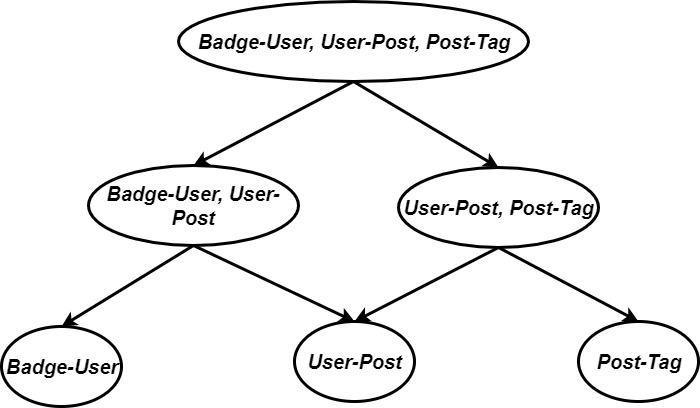
\includegraphics[scale=0.6]{pic/Structurelattice.jpg}
\caption{A substructure lattice with \textit{Badge-User, User-Post, Post-Tag} as its root node.}
\label{fig:4:3}
\end{figure}


Line 2-4 initializes covered substructures for each previous query as empty. For a previous query, $coveredSubstructure$ keeps what substructures have been selected so far which are useful for processing this query. It will be updated each time a new substructure is selected.
Line 5-12 performs ``score calculation'' in ``greedy selection framework''. For each substructure, Line 6 estimates its space. Line 8-10 iterates over all ``favored'' previous queries (favored by current substructure) and adds on marginal benefit (if any). Here marginal benefit refers to the time saved after adding current substructure to selected substructures (Line 9). Line 13-23 performs ``pick-and-update'' in ``greedy selection framework''. Line 15-17 terminates selection when there is no marginal benefit any more. Line 19-22 updates covered substructures for previous queries as a result of current round of selection.

Implementation of functions are listed as follows. Again users can implement these functions in their own ways based on their database systems. Function \textit{space(substructure)} returns estimated space cost of a substructure materialization. We use Neo4j's execution plan API to get estimated result size of a substructure. Function \textit{benefit(q, substructure, q.coveredSubstructres)} evaluates marginal benefit of substructure to query $Q$ when substructures in $q.coveredSubstructres$ have been materialized. We know that execution plan and estimated intermediate result size are provided by Neo4j's API. But such information is on database's naive processing plan. When substructure materialization is used, execution plan (intermediate result) becomes different from naive processing plan. As a result estimation on marginal benefit of a substructure is tricky. We use $time(q.coveredSubstructres \cup substructure)$ - $time(q.coveredSubstructres)$ for estimation of marginal benefit of a substructure. We think that this roughly indicates overall improvement of adding $substructure$ to $coveredSubstructres$ as materializations.



%----------------------------------------------------------------------
\subsection{ID and Property Selection}
%----------------------------------------------------------------------

Given a substructure picked by Structure Planner, we need to decide on which IDs and properties should be stored. Keeping all IDs and attributes makes a substructure materialization more informative but increases space cost. We are faced with a trade-off between space cost and usage potential. Selection on IDs and properties is an important issue. We will use substructure \textit{User-Post, Post-Tag} as an example and discuss different ID and property selection policies.

For IDs, we consider the following two policies.

\begin{itemize}
\item Policy \#1 keeps IDs of all nodes and edges. This enables ``overlap'' join with other substructures but increases space cost. For \textit{User-Post, Post-Tag}, if we keep IDs of all nodes and edges, then we can perform join operation with \textit{Badge-User, User-Post}. We call such join an ``overlap'' join as the two substructures have an overlap part which is \textit{User-Post}. Note that we can join the two substructures only when IDs of nodes (User and Post), and edge (edge between User and Post) are stored in both substructures.

\item Policy \#2 only keeps IDs of ``border nodes'' which are on the border of the substructure's \textit{structure}. Figure \ref{border node} highlights ``border nodes'' of structure \textit{User-Post, Post-Tag}. In this example we only save IDs of User and Tag. We do not keep IDs of Post as node Post is not located on the border of the \textit{structure}. Compared to Policy \#1, this saves space cost but ``overlap join'' with other substructures is not enabled. Policy \#2 only enables joins on border nodes. For example we may join \textit{User-Post, Post-Tag} with \textit{User-Badge} on their common border node User.

\begin{figure}[H]
\centering
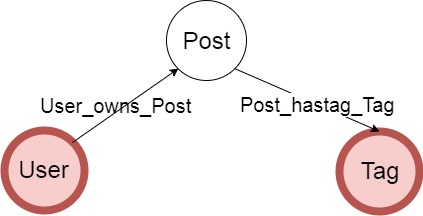
\includegraphics[scale=0.7]{pic/bordernode.jpg}
\caption{``Border nodes'' of structure \textit{User-Post, Post-Tag}.}
\label{border node}
\end{figure}
\end{itemize}


We use Policy \#1 in our implementation. However if keeping IDs of inner nodes and edges overwhelmingly increases result length, it's wise to choose Policy \#2 as space cost becomes too high. 

For properties, we consider the following two policies.

\begin{itemize}
\item Policy \#1 keeps all properties.
\item Policy \#2 only keeps properties that were queried in previous workloads.
\end{itemize}

Our suggestion is to consider the proportion of properties which were queried in previous workload over all properties in the data schema. For example, in our experiment only a small proportion of properties were queried. We choose Policy \#2 as it is a waste of space to keep all properties. 


%----------------------------------------------------------------------
\section{Query Processing}
\label{Future Query Processing Part}
%----------------------------------------------------------------------
Future Query Processing Part aims at processing future queries efficiently using substructure and cuboid materializations. When future query $Q$ arrives, we first consult cuboids materializations. If $Q$ can be answered by aggregation over any cuboid materializations, we select the cuboid with minimum space and directly scan over it to produce result of $q$. If $Q$ cannot be answered by any cuboid, we decompose $Q$ and use substructures to compose the result of $q$. 

\begin{algorithm}[H]
\caption{FutureQueryProcessing}
\LinesNumbered
\textbf{System:} C: a set of materialized cuboids\\ S: a set of materialized substructures\\ 
\KwIn{q: a query\\}
\KwOut{r: result of q}

$minspace:= \infty $\;
mincuboid := NULL\;
\ForEach{$cuboid \in C$}{
\If{cuboid.structure = q.structure and q.dimension \subseteq cuboid.dimension}{
	\If{$cuboid.space<minspace$}{
		minspace := cuboid.space\;
		mincuboid := cuboid\;
	}
}

\eIf{$mincuboid \not= NULL$}{
	$r := aggregate(mincuboid, q)$\;
}{
	$r :=Decompose\_Join(q)$\;
}
}
\end{algorithm}
\clearpage

Line 4-9 looks up materialized cuboids and find if any cuboid can be used to answer query $q$. If there are multiple useful cuboids we use the cuboid with the smallest scanning cost ($cuboid.space$). Note that $cuboid.space$ was computed in Line 9 in Algorithm SingleCubePlanner in Section \ref{SingleCubePlanner}. Line 10 checks if $q$ can be answered by cuboid materializaiton. If yes we perform aggregation operation over the cuboid (Line 11). Otherwise we need to decompose $q$ into substructures and compose the result (Line 13). Function $aggregate(mincuboid, q)$ is classic aggregation operation. We will discuss how function $Decompose\_Join(q)$ is implemented in the following subsections. 

%----------------------------------------------------------------------
\subsection{Substructure Selection}
\label{Substructure Selection}
%----------------------------------------------------------------------

Before discussion on $Decompose\_Join(q)$, we need to first solve a ``Substructure Selection'' problem. In order to decompose a query $q$, we need to consider which materialized substructures we need to use. We need to make dicision when candidate substructures in $S$ overlap. For example suppose $q$ has structure \textit{Badge-User, User-Post, Post-Tag}.

And S consists of substructures 

(1)Badge-User

(2)Badge-User, User-Post 

(3)User-Post, Post-Tag

(4)Post-Tag

(5)User-Post.

We can get structure of $q$ by joining structures of (1) and (3). Thus (1) and (3) seems to be a possible combination for substructure selection in this case. Actually we may have at least three ways of substructure selection: (1) and (3); (2) and (4);
(1), (4) and (5). The key question is which selection will result in fastest processing time on $q$? Here are some intuitions to solve this tricky question. First, when we select substructures one by one, we do not select a substructure when it is covered by selected substructures. For example we will not consider (1) if (2) has been selected as (1) is covered by (2). Second, we prefer to minimize total size of selected substructures as we need to at least access each selected view once. We prefer less memory access. Third, we prefer smaller number of selected substructures as intuitively this causes less times of joins. 

We propose a greedy algorithm for substructure selection based on user defined heuristics. Users may define heuristic functions based on intuitions (like the three intuitions mentioned above). The idea of the greedy algorithm is to always pick up next substructure with highest  score of user defined heuristic function $h(s)$, which returns heuristic score for a substructure $s$. Some exampling heuristics are \#edges of substructure, score calculated in StructurePlanner (Line 11 in Algorithm StructurePlanner), table size etc. 

\begin{algorithm}[H]
\caption{SelectSubstrucre}
\LinesNumbered
\textbf{System:} S: a collection of materialized substructures\\ h(s): user defined function. It returns heauristic score of a substructure $s$.\\
\KwIn{q: a future query\\}
\KwOut{V : selected views for future joining\\ uncoveredStruc: structure not covered by selected views\\uncoveredProp: properties not covered by selected views\\}
uncoveredStruc := q.structure\;
uncoveredProp:= q.properties\; 
$coveredStruc:= \emptyset$\;
$V:=\emptyset $\;
\ForEach{$s \in S$ ordered by h(s)}{
\If{s $\subseteq$ uncoveredStruc and s $\not\subseteq$ coveredStruc}{
	$V := V \cup \{s\}$\;
	$coverdStruc := coveredStruc \cup s.structure$\;
	uncoveredStruc := uncoveredStruc - s.structure\;
	uncoveredProp := uncoveredProp -s.properties\;
}
}
\end{algorithm}
\clearpage

Line 1-2 initializes $uncoveredStruc$ and $uncoveredProp$, which keeps track of structures and properties which have not been covered by selected substructures. Such uncovered structures and properties will need to be fetched from database. Line 3 initializes $coveredStruc$, which keeps union of selected substructures. Line 5 starts iteration over substructures ordered by user-defined heuristics $h(s)$. Line 6 assures that a candidate substructure that is totally covered by selected substructures will be disqualified. In the above example, suppose we have already selected (2), there is no need to select (1) since (1) is totally covered by (2). 

%----------------------------------------------------------------------
\subsection{Decomposition and Join}
\label{Query Decomposition}
%----------------------------------------------------------------------
We have talked about how to select substructure materializations in last subsection. In this part, we will finally discuss how to implement function $Decompose\_Join(q)$ (as in Algorithm FutureQueryProcessing in subsection \ref{Future Query Processing Part}). Besides $Decompose\_Join(q)$, we shall discuss two other variations of implementation: $Decompose\_Join_{informative}$ and $Decompose\_Join_{decisive}$. 

%----------------------------------------------------------------------
\subsubsection{\#1 $Decompose\_Join$}
%----------------------------------------------------------------------
Given a query $q$, we use the previously discussed algorithm ``SelectSubstrucre'' to select a set of substructure materializaions $V$. However, substructures in $V$ may not completely covers the structure of $V$. If there is any remaining structure ($uncoveredStruc$) and properties ($uncoveredProp$) that $V$ does not cover, we need to retrieve them from database. We call such remaining structure and properties fetched from database ``complementary  components''. After all these components (both materializations and ``complementary  components'') are finally ready, we join and aggregate them together to produce final results.

\begin{algorithm}[H]
\caption{Decompose\_Join}
\LinesNumbered
\textbf{System:} S: a collection of materialized substructures\\ heuristic: heuristic for ordering S\\
\KwIn{q: a future query\\}
\KwOut{r: result of q}
$\Sigma \gets \emptyset $\;
$V, uncoveredStruc, uncoveredProp \gets SelectSubstrucre(q) $\;
$\Sigma \gets \Sigma \cup V $\;
Splits:=split(uncoveredStruc, uncoveredProp)\;
\ForEach{s: Splits}{
$\Sigma \gets \Sigma \cup \{retrieve(s)\} $\;
}
r := join\_aggregate(\Sigma, q)\;
\end{algorithm}

Line 1 initializes $\Sigma$, which maintains a set of all components (materializations and ``complementary  components'') that are needed. Line 2 selects substructures using SelectSubstructure algorithm. $uncoveredStruc$ and $uncoveredProp$ refer to structures and properties which are not covered by selected substructures. They are ``complementary components'' and will be retrieved from database servers. Line 4 splits $uncoveredStruc$ and $uncoveredProp$ into connected components. We will retrieve each connected component from database server. Note that splitting is necessary since $uncoveredStruc$ may not be exactly one connected component. Line 8 joins and aggregates all materials together to produce results. 

Function \textit{split(uncoveredStruc, uncoveredProp)} is implemented by classic connected components detection algorithms. It splits $uncoveredStruc$ and $uncoveredProp$ into connected components (structures). We want to retrieve each connected structure seperately from database because otherwise it may result in unnecessarily large results of cartesian products of several disconnected structures. Function \textit{$materialize(s)$} retrieve ``complementary components'' $s$ from database server. Function \textit{join($\Sigma$, q)} join tables of $\Sigma$ together and aggregate over properties based on $q$. Joins over multiple tables has been a well-studied topic. Joining order and join technique (hash join etc) are two important aspects on this topic. In our implementation we use hash join and our joining order policy is to keep joining two tables which have minimum sum of table sizes and have common column(s). That is, we tend to select two smaller tables to join.  

%----------------------------------------------------------------------
\subsubsection{\#2 $Decompose\_Join_{informative}$}
%----------------------------------------------------------------------
$Decompose\_Join$ retrieve ``complementary components'' from database in a naive manner. We adopt the idea of Semi-Join \cite{DBLP:journals/dr/Ozsoyoglu99} and propose anther way of implementation: $Decompose\_Join_{informative}$. Semi-join takes advantage of ``selection'' effect of natural join. In $Decompose\_Join_{informative}$, we first perform joins over substructures of $V$. When we retrieve ``complementary components'' from database server, we inform database server with sets of candidate node and edge IDs as a result of joins over $V$. We name this approach $Decompose\_Join_{informative}$ as instead of naively query ``complementary components'' from database, we try to inform database server with sets of candidate IDs. Database backend only needs to search within candidate IDs.

\begin{algorithm}[H]
\caption{$Decompose\_Join_{informative}$}
\LinesNumbered
\textbf{System:} S: a collection of materialized substructures\\ heuristic: heuristic for ordering S\\
\KwIn{q: a future query\\}
\KwOut{r: result of q}
$\Sigma \gets \emptyset $\;
$V, uncoveredStruc, uncoveredProp \gets SelectSubstrucre(q) $\;
V^{*}:=join(V)\;
$\Sigma \gets \Sigma \cup V $\;
Splits:=split(uncoveredStruc, uncoveredProp)\;
\ForEach{s: Splits}{
$\Sigma \gets \Sigma \cup \{retrieve\_{informative}(s, V^{*})\} $\;
}
r := join\_aggregate(\Sigma, q)\;
\end{algorithm}
\clearpage

$Decompose\_Join$ performs joining after ``complementary components'' are prepared. Unlike $Decompose\_Join$, we first join $V$ in Line 3 before retrieval of ``complementary components'' from databases in Line 7. Note that substructures in $V$ may reside in multiple connected components. Thus $join(V)$ may come to a result of multiple intermediate tables.

In Line 7, $retrieve\_{informative}(s, V^{*})$ fetches results from databases by passing candidate IDs information (from join result $V^{*}$). Different database server may have different syntax to achieve this. In SQL we may pass candidate IDs using \textit{WHERE} statement. Neo4j supports query with a list of IDs as arguments in \textit{WHERE} statement.


\textbf{$Decompose\_Join_{informative}$ vs. $Decompose\_Join$}

\textit{Pros}: ``Informative materialization'' helps accelerate retrieval process from backend databases in two aspects. First, since screened out candidate IDs are provided, database backend only needs to iterate through a portion of nodes and edges. This will reduce database processing time. Second, candidate IDs has a filtering effect thus size of retrieval results is likely to be deducted. Thus time of result transmit will be reduced.

\textit{ Cons:} First, $Decompose\_Join_{informative}$ has an transmit overhead of IDs. Second, $Decompose\_Join$ performs one round of joins after all components are ready. $Decompose\_Join_{informative}$ performs first round of joins on $V$ before without ``complementary components'' are ready and then second round of joins. In terms of joining orders, $Decompose\_Join$ is better as its one-round joining order is based on all components with all possible orders of joining.

------------------
\subsubsection{\#3 $Decompose\_Join_{decisive}$}
%----------------------------------------------------------------------
We have mentioned two advantages of $retrieve\_{informative}(s, V^{*})$. However a disadvantage of $retrieve\_{informative}(s, V^{*})$ is an overhead of transport of candidate IDs. We propose a decisive way to evaluate the trade-off between overhead and benefits of $retrieve\_{informative}(s, V^{*})$ and choose between $retrieve\_{informative}(s, V^{*})$ and $retrieve(s)$.

\begin{algorithm}[H]
\caption{$Decompose\_Join_{decisive}$}
\LinesNumbered
\textbf{System:} S: a collection of materialized substructures\\ heuristic: heuristic for ordering S\\
\KwIn{q: a future query\\}
\KwOut{r: result of q}
$\Sigma \gets \emptyset $\;
$V, uncoveredStruc, uncoveredProp \gets SelectSubstrucre(q) $\;
V^{*}:=join(V)\;
$\Sigma \gets \Sigma \cup V $\;
Splits:=split(uncoveredStruc, uncoveredProp)\;
\ForEach{s: Splits}{
\eIf{decide\_informative(s,V^{*})}{
	$\Sigma \gets \Sigma \cup \{retrieve\_{informative}(s, V^{*})\} $\;
}{
	$\Sigma \gets \Sigma \cup \{retrieve(s)\} $\;
}
}
r := join\_aggregate(\Sigma, q)\;
\end{algorithm}
\clearpage

In Line 7, Function $decide\_informative(s,V^{*})$ makes decision between $retrieve\_{informative}(s, V^{*})$ and $retrieve(s)$. In our implementation we estimate result sizes two retrieval methods: $retrieve\_{informative}(s, V^{*}).estimatedSize$ and $retrieve(s).estimatedSize$. $retrieve(s).estimatedSize$ can be returned by space(substructure) in Algorithm ``StructurePlanner'' in subsection \ref{Structure Planner}. We calculate $retrieve\_{informative}(s, V^{*}).estimatedSize$ in the following way:

1. Randomly sample a small number of candidate IDs.  

2. Do $retrieve\_{informative}$ but passing only sampled candidate IDs. We call this a ``trial query''. We want to use ``trial query'' to estimate result length of actual $retrieve\_{informative}(s, V^{*})$. Since we only pass a small number of IDs, time cost of ``trial query'' is small.

3. Using result length of ``trial query'', calculate $retrieve\_{informative}(s, V^{*}).estimatedSize$ proportionally.

After $retrieve(s).estimatedSize$ and $retrieve\_{informative}(s, V^{*}).estimatedSize$ are calculated. We use 

$retrieve(s).estimatedSize - retrieve\_{informative}(s, V^{*}).estimatedSize / sizeOf(candidateIDs)$ and compare the ratio with a threshold to evaluate trade-off and make decision.

\textbf{$Decompose\_Join_{decisive}$ vs. $Decompose\_Join_{informative}$}: We see that $Decompose\_Join_{decisive}$ performs two rounds of joins like $Decompose\_Join_{informative}$. The major difference is that $Decompose\_Join_{decisive}$ plays ``trial query''. The principle behind ``trial query'' is to pay an acceptable price of time cost so that we make wise decision on ``complementary components'' retrieval. A good decision making on ``complementary components'' retrieval often saves much more time than time cost of ``trial queries'', especially when dataset is large. 




%----------------------------------------------------------------------



%======================================================================
\chapter{Evaluation}
%======================================================================
In this chapter, we validate our proposed solution with a set of meaningful queries over a real world dataset. To demonstrate the time efficiency of our approach, we select Neo4j community version 3.1.3 as the baseline. In the experiments, we test query processing time and space cost by running the queries using both our approach and Neo4j implementation.  The results show that our approach is about 20 times faster than the Neo4j implementation on average under the default settings (to be covered in Section \ref{Aspects of Interest}). Moreover, we assess and explain how each aspect in our system affects processing efficiency. Finally, we discuss our reflection on the Neo4j system.

%-------------------------------------------
---------------------------
\section{Experiment Setup}
%----------------------------------------------------------------------

%Our main focus is to evaluate different strategies for preprocessing and query evaluation. For instance, the threshold of “Is hot-structure” part in the diagram,  selection policy for materialized substructures in “Cube-Planner” and “Structure-Planner” , different heuristics when ranking sub-structures during decomposition in “Decomposition and Joining” etc.

There are two purposes of our experiments. First is to demonstrate the query processing efficiency of our proposed solution by comparing against the native Neo4j system. Second, we would like to test how different settings (of parameters and choices of strategies) in our solution affect query processing efficiency. %Experiments are run on a set of self-designed meaningful queries on a real-world dataset.

%----------------------------------------------------------------------
\subsection{Datasets}
%----------------------------------------------------------------------

We use the StackOverFlow dataset in our experiments that is generated by using raw information from https://archive.org/details/stackexchange. The dataset contains user-contributed content (such as user information, posts and etc.) on www.stackoverflow.com. The dataset contains 10 different node labels and 12 different edge labels.  Figure \ref{fig:metaexp} shows the meta graph of 8 node labels and 8 edge labels that are involved in our experiments. The data graph contains over 300 million vertices and more than 400 million edges and takes 44.5GB of storage.
\par

\begin{figure}[H]
	\centering
	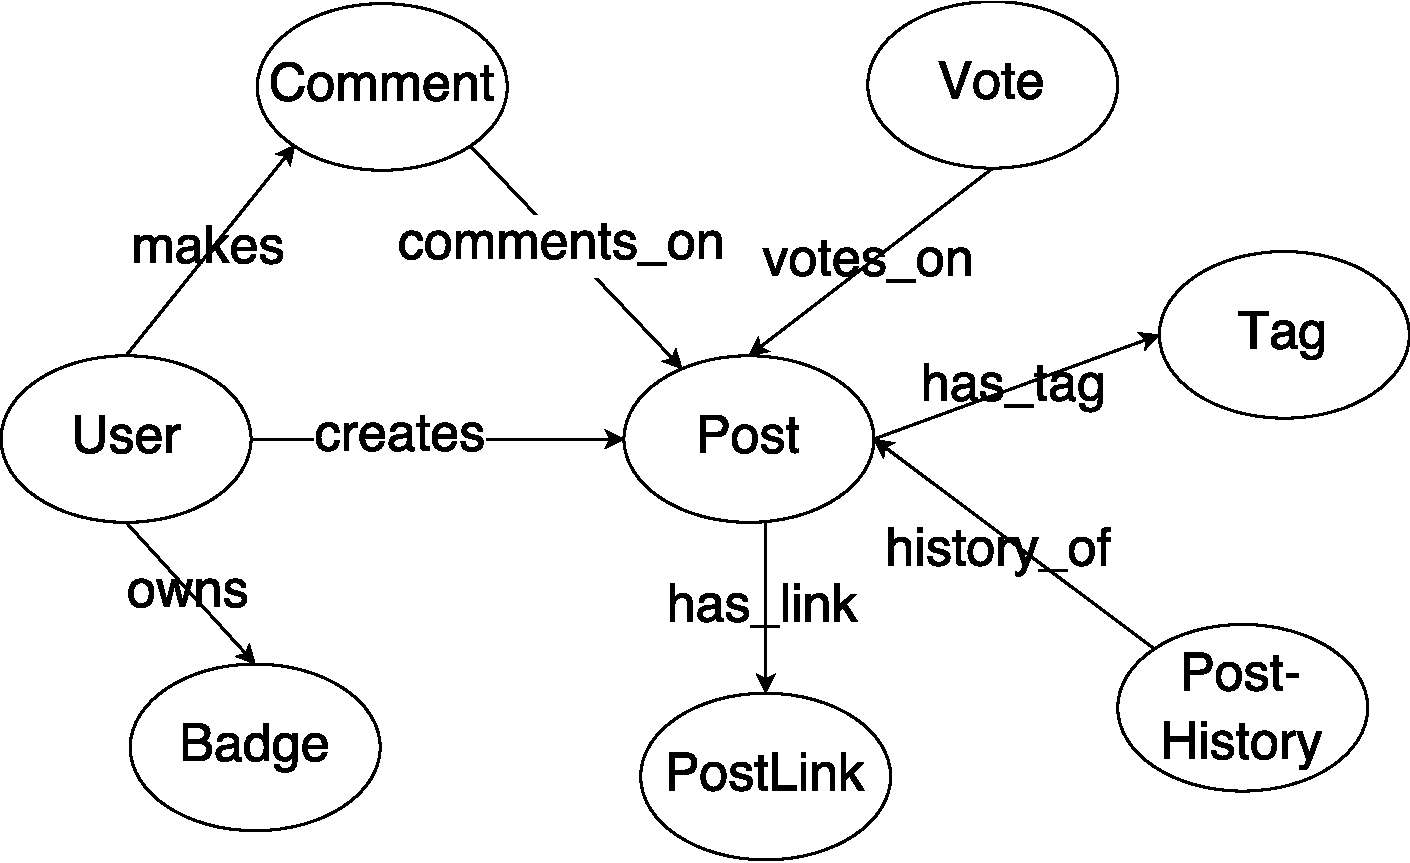
\includegraphics[scale=0.37]{pic/expmeta.pdf}
	\caption{The meta graph of StackOverFlow used in experiments.}
	\label{fig:metaexp}
\end{figure}

%\begin{figure}[H]
%	\centering
%	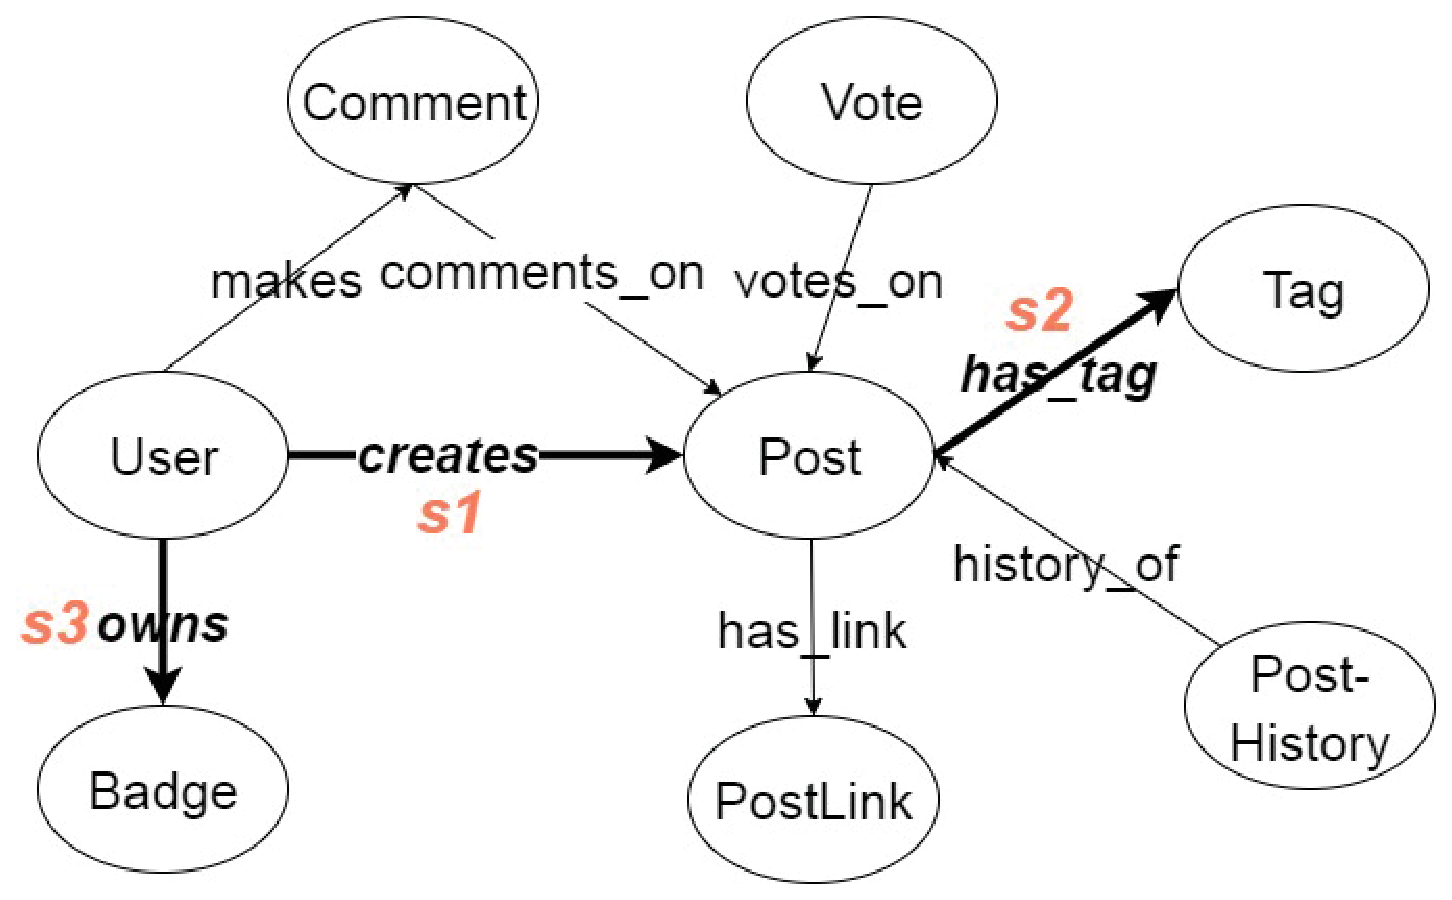
\includegraphics[scale=0.5]{pic/MetaExpS.eps}
%	\caption{The meta graph of StackOverFlow used in experiments.}
%	\label{fig:5:1}
%\end{figure}


%----------------------------------------------------------------------
\subsection{Query Workloads}
%----------------------------------------------------------------------
We design 24  queries against the StackOverFlow dataset given below. We randomly select 12 queries as the previous workload, leaving the rest 12 ones as the future workload.  %The meaning of each query is explained in the Appendix.


\textbf{Previous WorkLoad:}

P1 \hspace{3mm} User-Post: User.UpVotes, Post.Score=10

P2 \hspace{3mm} User-Post: User.UpVotes, (AVG)Post.Score

P3 \hspace{3mm} User-Post: User.Age, (SUM)Post.ActiveMonth

P4 \hspace{3mm} User-Post: User.CreationDate\_Year, Post.PostTypeId=1

P5 \hspace{3mm} Badge-User, User-Post, Post-Tag: Tag.TagName, User.CreationDate\_Year=2017

P6 \hspace{3mm} Badge-User, User-Post, Post-Tag: Tag.TagName, Badge.Name

P7 \hspace{3mm} Badge-User, User-Post:Badge.Date\_Year, (AVG)Post.Score

P8 \hspace{3mm} Badge-User, User-Post:Badge.Class, (AVG)Post.ActiveMonth

P9 \hspace{3mm} User-Post, Post-Tag: (AVG)User.Age, Tag.TagName

P10 \hspace{1.3mm} User-Post, Post-Tag: (AVG)User.UpVotes, Tag.TagName=Java

P11 \hspace{1.3mm} User-Post, Post-Vote: (AVG)User.UpVotes, Vote.VoteTypeId

P12 \hspace{1.3mm} Post-Comment, Post-PostLink: PostLink-LinkTypeId, (AVG)Comment-Score


\par
\textbf{Future WorkLoad:}

Q1 \hspace{3mm} User-Post: User.CreationDate\_Year=2017, Post.PostTypeId

Q2 \hspace{3mm} User-Post: (AVG)User.UpVotes,Post.Score

Q3 \hspace{3mm} User-Post: Post.ActiveMonth, (AVG)User.Age

Q4 \hspace{3mm} User-Post: User.CreationDate\_Year

Q5 \hspace{3mm} Badge-User, User-Post, Post-Tag: Tag.TagName, Badge.Class

Q6 \hspace{3mm} Badge-User, User-Post, Post-Tag: Tag.TagName, Badge.Date\_Year

Q7 \hspace{3mm} Badge-User, User-Post:Badge.Name, Post.PostTypeId

Q8 \hspace{3mm} User-Post, Post-Tag: User.UpVotes, Tag.TagName, Post.PostTypeId=2

Q9 \hspace{3mm} User-Post, Post-Tag:User.CreationDate\_Year, Tag.TagName

Q10 \hspace{1.3mm} Badge-User, User-Comment: Badge-Class, (AVG)Comment-Score

Q11 \hspace{1.3mm} Badge-User, User-Comment: Badge-Name, (AVG)Comment-Score

Q12 \hspace{1.3mm} Post-PostHistory, Post-Tag: Tag-TagName, PostHistory-PostHistoryTypeId





%----------------------------------------------------------------------
\subsection{System Setting}
%----------------------------------------------------------------------

We run the experiments on a Linux server with 256GB main memory. Our system is implemented in Java. We set the initial JVM memory to 100GB, and the maximal JVM memory to 200GB.

Our solution is developed on top of Neo4j Community v3.1.3. In the experiment, we set Neo4j's initial memory as 60GB and 200GB for the maximum usage. We use Neo4j's official Java driver (https://neo4j.com/developer/java/\#neo4j-java-driver) to interact with Neo4j server.

%----------------------------------------------------------------------
\section{Aspects of Interest}
\label{Aspects of Interest}
%----------------------------------------------------------------------

As we mentioned, there are two purposes of our experiments. In addition to the efficiency test, we would like to study how different settings in our system could affect query processing efficiency. We list the following aspects of interests to be tested. Default setting for each aspect is also presented. 

\textbf{Materialization}
\begin{itemize}
	
	\item  Space cost limit ($\sigma$ in Algorithm \ref{alg:StructurePlanner} in Section \ref{Structure Planner}) is set to 6GB by default. Results and discussion are presented in Section \ref{Space Cost Limit}.
	
	\item  Algorithms in materialized view selection described in Section \ref{Materialization Part}. For cuboid selection, we compare CubePlanner (in Section \ref{sec:CubePlanner}) with the ``Partial Materialization'' algorithm (PMA) proposed in Graph Cube \cite{sigmod11_ZhaoLXH11}. For substructure selection we will compare StructurePlanner (in Section \ref{Structure Planner}) with the well-known maximal frequent pattern mining algorithm (FPM) \cite{DBLP:conf/icdm/GoudaZ01}. In other tests, CubePlanner and StructurePlanner are used by default. Results are discussed in Sections \ref{CubePlannerPMA} and \ref{StructurePlanner vs FPM}, respectively.
	
	\item Frequency threshold for identification of “hot structures” ($\omega$ in Algorithm \ref{alg:1}). We set the default value to be 4; the intuition of default value, together with results and discussion are elaborated in Section \ref{Frequency Threshold}.
	
	\item Storage level for materialized views. We  compare main memory storage vs hard disk storage. Note that memory based materialization is set as the default in all other tests. Detailed discussion is provided in Section \ref{Storage Level for Merialized Views}.
	
\end{itemize}

\textbf{Future Query Processing}
\begin{itemize}
	\item  Choice of score functions in ranking substructures during the  ``Substructure Selection'' ($h(s)$ in Algorithm \ref{alg:SelectSubstrucre} discussed in Section \ref{Substructure Selection}). By default, $h(s)$ returns the score of $s$ calculated in StructurePlanner (as result of line 11 in Algorithm \ref{alg:StructurePlanner}). Results and explanations can be found in Section \ref{exp:Substructure Selection}.
	
	\item  Choice among using $Decompose\_Join$, $Decompose\_Join^{*}$ and $Decompose\_Join^{+}$ in ``Decomposition and Join'' in Section \ref{Query Decomposition}. We use $Decompose\_Join$ as the default method. Detailed discussion is in Section \ref{exp:DecomposeJoin}.
	
\end{itemize}

%Besides, we also ran experiments on the smaller dataset to see how performance varies in datasets of different sizes.

%----------------------------------------------------------------------
\section{Results and Discussion}
\label{Results and Discussion}
%----------------------------------------------------------------------
Following the interests of study listed above, we now present our experimental results.

%----------------------------------------------------------------------
\subsection{Our System vs. Neo4j}
\label{Our System vs. Neo4j}
%----------------------------------------------------------------------
We first show the time efficiency of our solution running in default settings against the native Neo4j implementation for the future workload.


\begin{figure}[H]
	\centering
	\includegraphics[scale=0.5, angle=270]{plot/neo4j.eps}
	\caption{Time efficiency on the future workload: our solution vs Neo4j.}
	\label{fig:neo4j}
\end{figure}

Figure \ref{fig:neo4j} shows the processing time for 12 future queries by both our system and Neo4j. Note that execution time for Q1 and Q4 in our system is 0.001s, and Neo4j does not finish processing Q5 and Q6 in 18 hours so we terminate execution and record the processing time as 18 hours. It is worth pointing out that with an extra 5.7GB space cost for materialized views, our solution achieves remarkable efficiency improvement. Given the size of our dataset, this extra space is acceptable.

\begin{figure}[H]
	\centering
	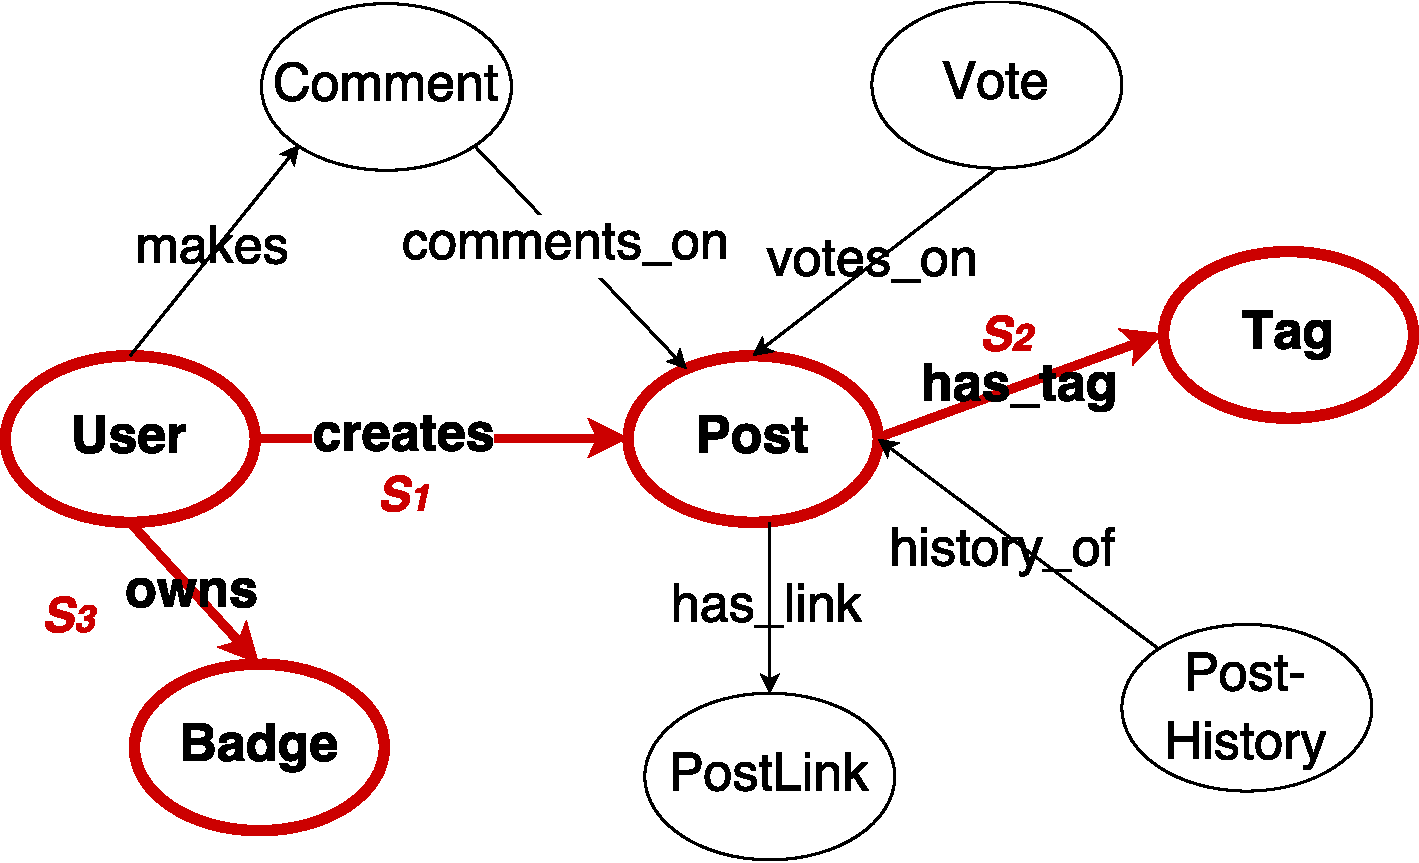
\includegraphics[scale=0.37]{pic/expmetaS.pdf}
	\caption{Substructure selected by StructurePlanner.}
	\label{fig:metagraphexperimenthot}
\end{figure}

We now detail how our system works over the 12 queries. First, \textit{User-Post} is identified as a ``hot structure'' as its frequency count is larger than or equal to the frequency count threshold. As a result, P1 - P4 are passed to the CubePlanner and P5 - P12 are passed to the StructurePlanner. Cuboids selected by CubePlanner are \{User.Age, Post.ActiveMonth\}, \{User.CreationDate\_Year, Post.PostTypeId\}, and \{User.UpVotes, Post.Score\}. Figure \ref{fig:metagraphexperimenthot} highlights substructures $S$ that StructurePlanner selects:  \textit{User-Post} ($s_1$), \textit{Post-Tag} ($s_2$) and \textit{Badge-User} ($s_3$). From the observation of the previous workload, we can tell that the StructurePlanner makes a good decision as these three substructures are able to cover most of previous queries.

We further explain the performance variance of the future workload. Overall improvement rate for Q1 - Q4 is more than 20000. This is because Q1 - Q4 are answered with a ``cuboid hit''. As a result, the time saving for these 4 queries are much greater than for Q5 - Q12 (which do not get a ``cuboid hit''). It worth pointing out that time complexities of cuboid aggregation and substructure joins are much different. The time complexity of a cuboid aggregation is bounded by the size of the Cartesian product of its dimensions. When it comes to substructure joins, however, the time complexity is related to the actual data sizes. Note that Q5 - Q9 are totally covered by $S$. In these cases, no ``complementary components'' are fetched from the Neo4j database.  Q10 - Q12 are partially covered by $S$.  Therefore, ``complementary components'' are fetched from the database, where a series of I/O operations increases the total time cost.  Overall, the overall improvement rate for Q5 - Q9 is around 40 times, while improvement rate for Q10 - Q12 ranges around 15 times. Clearly, our system could greatly improve query processing efficiency with an acceptable incremental space cost. While the improvement ratio varies in different scenarios of cuboid and structure ``hits''.




%----------------------------------------------------------------------
\subsection{Frequency Threshold}
\label{Frequency Threshold}
%----------------------------------------------------------------------
Frequency threshold $\omega$ can significantly affect the query processing efficiency. A change of $\omega$ may result in different ``hot structures'', followed by varied inputs for the CubePlanner and the StructurePlanner. It would further lead to different materialized view selection and overall query processing performance. As indicated in Section \ref{Overview of Materialization Part}, $\omega$ serves as a minimum threshold for building a cuboid over a ``hot structures'' (``cuboid hit'' assured). We think 4 is an appropriate choice for $\omega$ in our test case considering the frequency count of structures in previous workload (as shown in the table below).

\begin{center}
	\begin{tabular}{ | c | c |}
		\hline
		Structure	&Frequency	\\ \hline
		\textbf{User-Post} 	&\textbf{4} \\ \hline
		Badge-User, User-Post, Post-Tag 	&2 \\ \hline
		Badge-User, User-Post	&2 \\ \hline
		User-Post, Post-Vote	&2 \\ \hline
		User-Post, Post-Vote	&1 \\ \hline
		Post-Comment, Post-PostLink	&1 \\ \hline
	\end{tabular}
	\end {center}
	
	Suppose we lower $\omega$ to 2. \textit{Badge-User, User-Post, Post-Tag} will be ``hot structure''. As a result, cuboid selection over \textit{Badge-User, User-Post, Post-Tag} will be considered based on merely two queries (P5 and P6). Notice that Q5 and Q6, which have structure \textit{Badge-User, User-Post, Post-Tag}, will never get ``cuboid hit''. This is because properties Badge-Class in Q5 and Badge-Date\_Year in Q6 do not even appear in P5 and P6. That is to say, in this case any cuboid selected over \textit{Badge-User, User-Post, Post-Tag} will be useless. In addition, when $\omega$ is set to 2, input for StructurePlanner will be only two queries (Q11 and Q12). Note that structure frequency counts of these two queries are both 1. In other words, these are the most ``random'' queries. Note that the idea of StructurePlanner is to discover of useful substructures based on a sufficient number of ``less hot'' queries. In this case, two ``random'' queries are not the ideal input for the StructurePlanner.
	
	Suppose we increase $\omega$ to 5; then there will be no cuboid that is materialized in our test case. As a result Q1 - Q4 will be processed using substructure materialization ($s_1$). Although it is still faster than the native Neo4j system, the outstanding improvement ratio of ``cuboid hit'' cannot be achieved.
	
	Figure \ref{fig:omega} presents the total processing time under different settings of $\omega$. Note that no structure has frequency count of 3, therefore setting $\omega$ as 3 and 4 would categorize the same set of ``hot structures’’ and thus yield the same materialized views. We reach the conclusion that $\omega$ does have a significant effect over the system performance. Actually, determination on the value of $\omega$ is an interesting classification problem (based on the frequency count), which is left as future work since it is not the main focus of this thesis.
	
	\begin{figure}[H]
		\centering
		\includegraphics[scale=0.5, angle=270]{plot/omega.eps}
		\caption{Total processing time under different settings of $\omega$.}
		\label{fig:omega}
	\end{figure}
	
	
	%----------------------------------------------------------------------
	\subsection{Space Cost Limit}
	\label{Space Cost Limit}
	%----------------------------------------------------------------------
	As pointed out in Section \ref{Our System vs. Neo4j}, the space cost of our materialized views is 5.7GB, while the default space cost, $\sigma$, is set to 6GB. In this section, we study the effect of $\sigma$ on the query processing efficiency.  Figure \ref{fig:limit} shows how the total processing time varies with different space costs (which were caused by setting $\sigma$ to 6GB, 4GB, and 2.5GB, respectively). Apparently,  with more views being materialized, the total processing time decreases. However, the marginal benefit from materializing more views also decreases. This indicates that our Greedy Selection Framework (in Section \ref{s:Greedy Selection Framework}) successfully picks the proper candidates according to marginal benefits they would bring.
	
	\begin{figure}[H]
		\centering
		\includegraphics[scale=0.5, angle=270]{plot/limit.eps}
		\caption{Efficiency vs Space Cost}
		\label{fig:limit}
	\end{figure}
	
	%----------------------------------------------------------------------
	\subsection{Storage Level for Materialized Views}
	\label{Storage Level for Merialized Views}
	%----------------------------------------------------------------------
	As listed in Section \ref{Aspects of Interest}, by default, materialized views are stored as objects in main memory. This guarantees fast data access on the cost of extra memory consumption. Alternatively, materialized views can be serialized and stored as files on hard disks. Figure \ref{fig:disk} shows a comparison of the total query processing time using memory-based views and disk-based views. As expected,hard disk storage does not perform as fast as main memory storage. However, it is worth noting that  the drop in efficiency is acceptable. Such a drop in efficiency is due to the I/0 overhead in loading materialized views from disk files.
	
	One interesting question is what is the point of storing materialized views in files, since eventually they are to be read into the main memory. Our answer is that in cases when main memory is far too small for holding all selected views, materialization on disk provides an alternative.
	
	\begin{figure}[H]
		\centering
		\includegraphics[scale=0.5, angle=270]{plot/disk.eps}
		\label{fig:disk}
		\caption{Main memory storage vs hard disk storage}
	\end{figure}
	
	%----------------------------------------------------------------------
	\subsection{CubePlanner vs PMA}
	\label{CubePlannerPMA}
	%----------------------------------------------------------------------
	We compare CubePlanner in Section \ref{CubePlanner} in our solution with PMA in Graph Cube \cite{sigmod11_ZhaoLXH11}. Figures \ref{fig:qjiawei} and \ref{fig:jiaweispace} show that CubePlanner outperforms PMA in both query processing efficiency and space cost. Cuboids selected by CubePlanner are $\{$User.Age, Post.ActiveMonth$\}$, $\{$ User.CreationDate\_Year, Post.PostTypeId$\}$, and $\{$User.UpVotes, Post.Score$\}$. While PMA selected $\{$User.Age, User.UpVotes, User.CreationDate\_Year, Post.PostTypeId, Post.Score, Post.ActiveMonth$\}$, $\{$User.Age, User.UpVotes, User.CreationDate\_Year, Post.PostTypeId, Post.ActiveMonth$\}$, $\{$User.Age, User.UpVotes, User.CreationDate\_Year, Post.PostTypeId, Post.Score$\}$.


\begin{figure}[H]
	\centering
	\includegraphics[scale=0.43, angle=270]{plot/qjiawei.eps}
	\caption{Time: CubePlanner vs PMA}
	\label{fig:qjiawei}
\end{figure}

\begin{figure}[H]
	\centering
	\includegraphics[scale=0.43, angle=270]{plot/jiaweispace.eps}
	\caption{Total cuboid space cost: CubePlanner vs PMA}
	\label{fig:jiaweispace}
\end{figure}

Both two approaches are considered as implementations of the Greedy Selection Framework given in Section \ref{s:Greedy Selection Framework}. The differences between the two implementations. CubePlanner uses the ratio of marginal benefit over space cost as a score for candidate ranking (line 11 in Algorithm \ref{alg:SingleCubePlanner}). While PMA only considers marginal benefit. That is to say, space cost is not taken into account in PMA. Moreover, PMA treats each combination of properties with an equal weight, regardless of how many times a combination has appeared in previous queries. For example, in our test case, the combination of {User.UpVotes, Post.Score} appears twice in previous workload. But PMA would treat {User.UpVotes, Post.Score} with the same weight as those combinations are not even queried in previous workload (\{User.UpVotes, Post.PostTypeId\} etc). As a result, CubePlanner adopts more information from previous workload and thus makes a better selection.

%----------------------------------------------------------------------
\subsection{StructurePlanner vs FPM}
\label{StructurePlanner vs FPM}
%----------------------------------------------------------------------
We compare our Algorithm \ref{alg:StructurePlanner} in StructurePlanner with FPM. In FPM we set the minimum support to 2 considering the frequency count as listed in the table in Section \ref{Frequency Threshold}. These two ways provide different substructure selections which lead to different processing efficiency. Figures \ref{fig:fpmtotal} and \ref{fig:fpmspace} show that our StructurePlanner outperforms FPM in both efficiency and space cost.

\begin{figure}[H]
	\centering
	\includegraphics[scale=0.43, angle=270]{plot/fpm.eps}
	\caption{Total processing time for future workload: StructurePlanner vs FPM}
	\label{fig:fpmtotal}
\end{figure}

\begin{figure}[H]
	\centering
	\includegraphics[scale=0.43, angle=270]{plot/fpm_space.eps}
	\caption{Space cost: StructurePlanner vs FPM}
	\label{fig:fpmspace}
\end{figure}

Figure \ref{fig:metagraphexperimenthot} highlights three selected substructures by StructurePlanner. As mentioned, it is a good selection as these three substructures are able to cover most of the previous queries. However, FPM selects \textit{Badge-User, User-Post, Post-Tag}, which is a bad selection because it is useful only for Q5 and Q6. In addition, materialization of \textit{Badge-User, User-Post, Post-Tag} results in even more space cost than materialization of the three edges separately (as selected by StructurePlanner). Figure \ref{fig:qfpm} details processing time for each query. FPM only outperforms StructurePlanner on Q5 and Q6. This is because Q5 and Q6 would be able to perform aggregation over the materialization of \textit{Badge-User, User-Post, Post-Tag} when FPM is applied. While table joins of $s_1$, $s_2$ and $s_3$ are required if StructurePlanner is applied, which clearly is more time consuming. However for Q7 - Q12, StructurePlanner is the winner as it gets at least a partial ``substructure cover'', while the FPM-selected structure is not helpful at all.

\begin{figure}[H]
	\centering
	\includegraphics[scale=0.5, angle=270]{plot/qfpm.eps}
	\caption{Processing time for each query: StructurePlanner vs FPM}
	\label{fig:qfpm}
\end{figure}


%----------------------------------------------------------------------
\subsection{Substructure Selection}
\label{exp:Substructure Selection}
%----------------------------------------------------------------------

In our experiment, $h(s)$ in Algorithm \ref{alg:SelectSubstrucre} does not make any difference during ``Substructure Selection''. This is because the three selected substructures do not share any edges. Note that scenarios in Section \ref{Substructure Selection} where multiple valid combinations of materialized substructures exist only happen when materialized substructures have overlaps.

%----------------------------------------------------------------------
\subsection{Decompose\_Join}
\label{exp:DecomposeJoin}
%----------------------------------------------------------------------
We now present the experiments comparing  $Decompose\_Join$, $Decompose\_Join^{*}$ and $Decompose\_Join^{+}$ in ``Decomposition and Join'' (presented in Section \ref{Query Decomposition}). Three different implementations in ``Decomposition and Join'' would lead to different processing performance for Q10 - Q12, as they are partially covered by $S$ and fetching ``complementary components'' from Neo4j is necessary. Figure \ref{fig:threeall} provides the processing time for Q10 - Q12 using the three approaches. $Decompose\_Join^{*}$ performs  better than $Decompose\_Join$ in Q10. This is because $Decompose\_Join^{*}$ passes to Neo4j candidate IDs of users who have badges, which provides a considerable ``filtering effect'' when fetching \textit{User-Comment}. As a result, $Decompose\_Join^{*}$'s processing time for fetching \textit{User-Comment} is reduced. Besides, its time for joining \textit{Badge-User} and \textit{User-Comment} also decreases because the table size of \textit{User-Comment} is smaller than that of $Decompose\_Join$, thanks to the ``filtering effect''. This is reflected in Figure \ref{fig:threejoin}, where the time for join is saved in $Decompose\_Join^{*}$. However $Decompose\_Join^{*}$ performs badly for Q12. This is because the ``filtering effect'' of \textit{Post-Tag} in fetching \textit{Post-PostHistory} is small as most posts have tags. In addition, $Decompose\_Join^{*}$ has an overhead of scanning the \textit{Post-Tag} table in order to get the set of candidate IDs. It explains why $Decompose\_Join^{*}$ takes longer time in processing Q12. Figure \ref{fig:threetotal} gives the total processing time for Q10 - Q12 using the three approaches. We see that $Decompose\_Join^{+}$ has best overall performance. To explain,  $Decompose\_Join^{+}$ is able to choose the faster approach when fetching ``complementary components'' from Neo4j in scenarios like Q10 and Q12 with  the cost of a cheap trial query (as discussed in Section \ref{Query Decomposition}). Note that the time cost for a ``trial query'' is bounded by a constant sample size, and is not proportional to actual data size in the dataset. A too small sample size results in bias in estimation, whereas a unnecessarily large sample size causes too much time cost. We tried different sample sizes and find  100 to be an appropriate value,  which serves estimation properly and saves the time cost. Figure \ref{fig:threesample} shows that the time cost ``trial query'' is negligible compared to the overall processing time.


\begin{figure}[H]
	\centering
	\includegraphics[scale=0.43, angle=270]{plot/threeall.eps}
	\caption{Processing time for Q10 - Q12 by three approaches.}
	\label{fig:threeall}
\end{figure}


\begin{figure}[H]
	\centering
	\includegraphics[scale=0.43, angle=270]{plot/threejoin.eps}
	\caption{Joining time in processing Q10 - Q12 by three approaches.}
	\label{fig:threejoin}
\end{figure}
\begin{figure}[H]
	\centering
	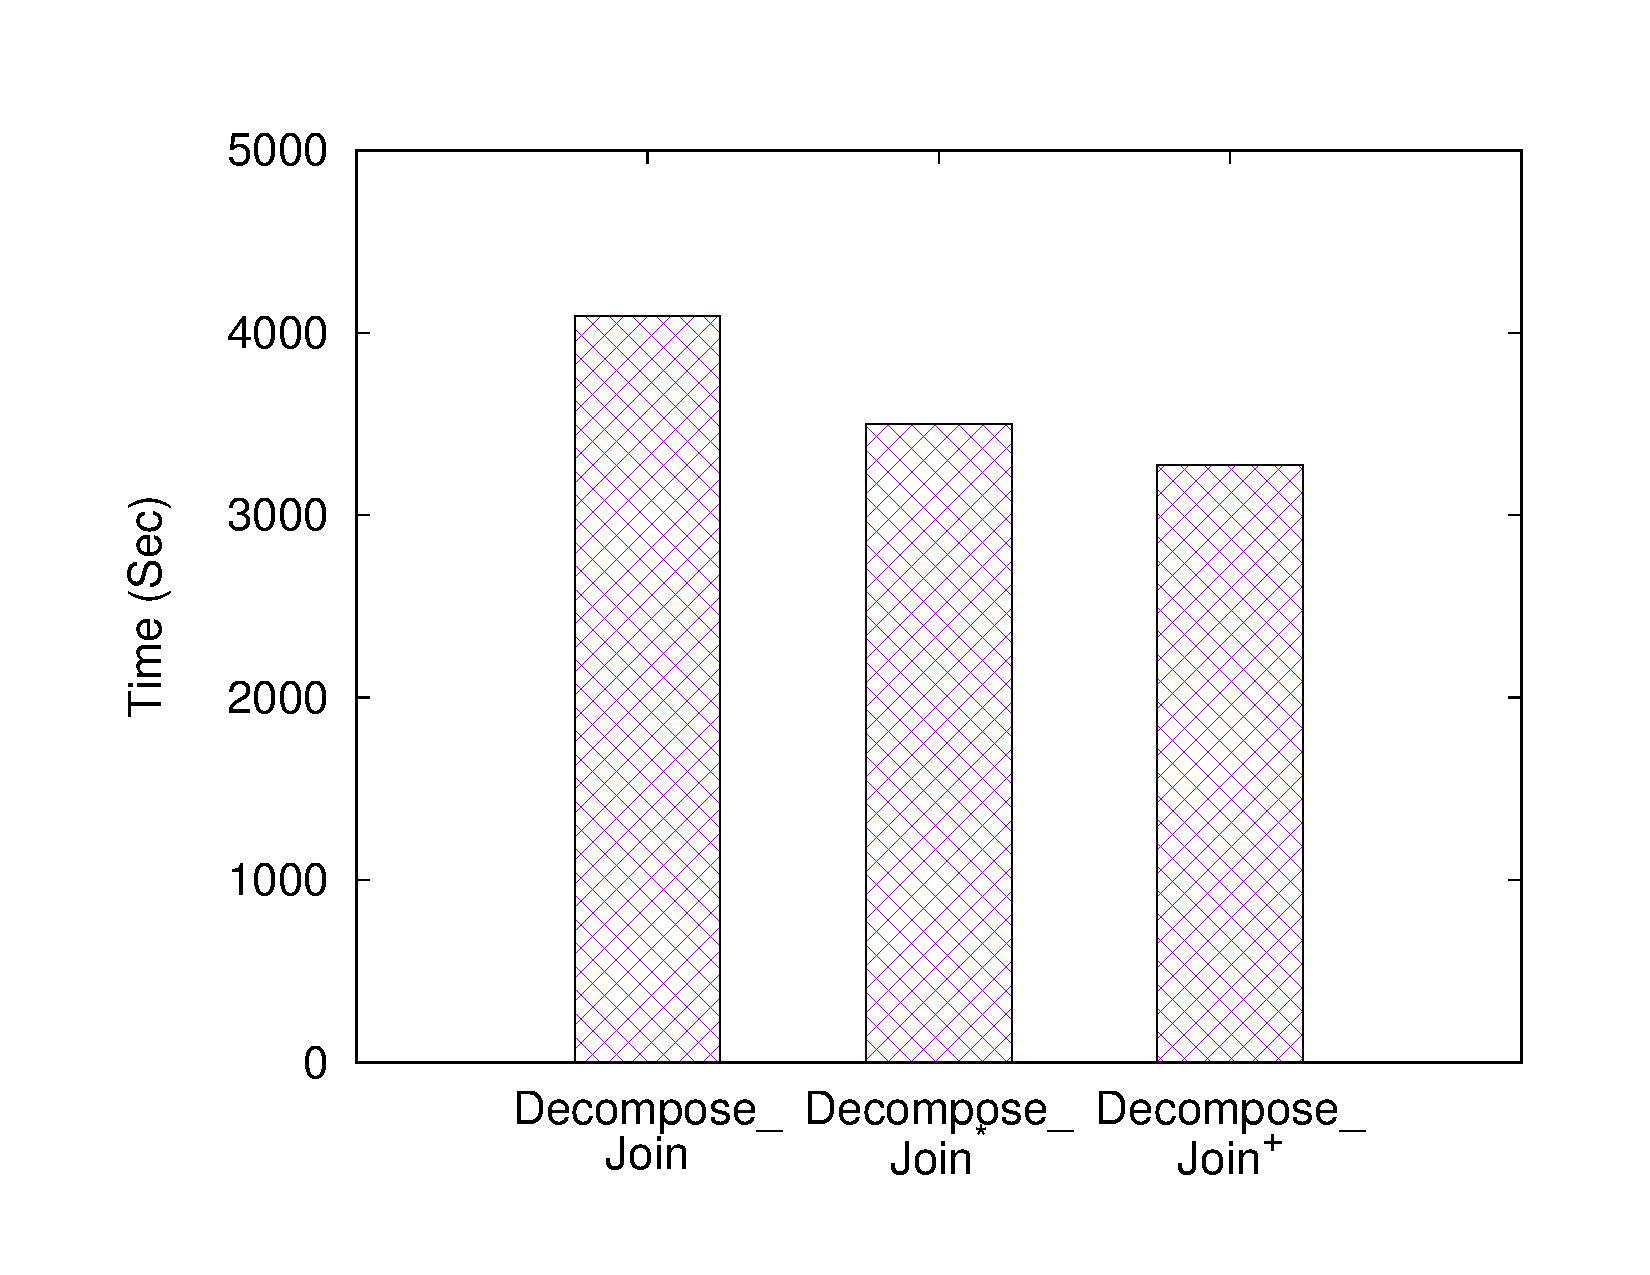
\includegraphics[scale=0.42]{plot/threetotal.pdf}
	\caption{Total processing time for Q10 - Q12 by three approaches.}
	\label{fig:threetotal}
\end{figure}

\begin{figure}[H]
	\centering
	\includegraphics[scale=0.42, angle=270]{plot/threesample.eps}
	\caption{Total processing time vs ``trial query'' processing time.}
	\label{fig:threesample}
\end{figure}

To conclude, ``filtering effect'' is an important factor in the performance of these three different implementations of ``Decomposition and Join''. In general, $Decompose\_Join^{+}$ is the recommended approach as it is able to select the better solution with a small cost of ``trial query''.


%%----------------------------------------------------------------------
%\subsection{Large DataSet vs Small DataSet (Only graphs not ready)}
%%----------------------------------------------------------------------
%Besides StackOverFlow dataset (45.8GB), we also tested on a smaller ``StackExchange-Math'' dataset of size 2.57GB. Like StackOverFlow dataset, StackExchange-Math dataset is about a mathematics Q\&A forum (https://math.stackexchange.com).  The raw data of StackExchange-Math dataset also comes from https://archive.org/details/stackexchange and it has exactly the same schema as StackOverFlow dataset.
%
%Figure \ref{} compares efficiency improvement rate for large dataset and smaller dataset. We see that our system achieved even better performance on larger dataset.

%----------------------------------------------------------------------
\subsection{Reflections on Neo4j}
%----------------------------------------------------------------------
During the experiments, we found that Neo4j uses a na\"ive approach to result size estimation for aggregation queries. It simply takes the square root of table length before aggregation as the estimated size for the aggregated result, regardless of which properties are being aggregated. Such a method leads to a huge bias in the estimation.

For example, Figure \ref{fig:wrong1} presents Neo4j's execution plans for queries \textit{User-Post: User.Age} and \textit{User-Post: ID(User), ID(Post)}, respectively. Obviously the latter query should have much larger estimated result size than the former one. However Neo4j returns exactly the same estimated result size by simply taking the square root of table length (216791 estimated rows in ``Projection'' step) in the previous step.

%explain match (u:User)-[]-(p:Post) return u.Age, count(*)

\begin{figure}[H]
	\centering
	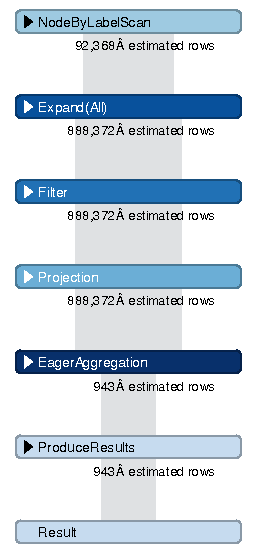
\includegraphics[scale=1.5]{pic/wrong.pdf}
	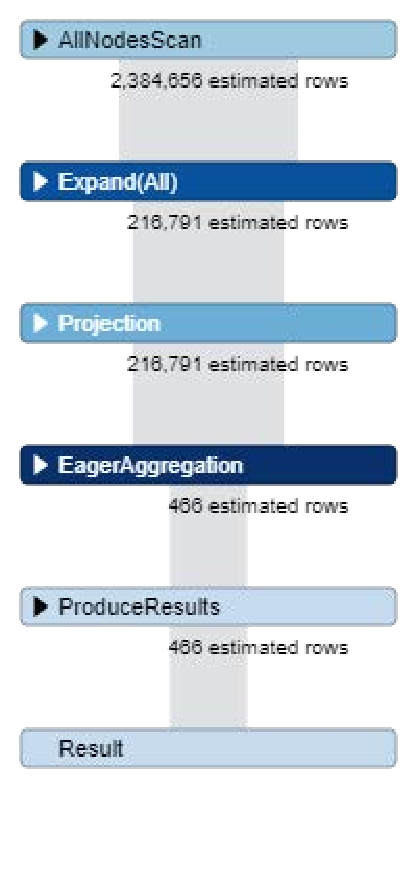
\includegraphics[scale=1.5]{pic/wrong2.pdf}
	\caption{Execution plans for \textit{User-Post: User.Age} and \textit{User-Post: ID(User), ID(Post)}.}
	\label{fig:wrong1}
\end{figure}

This is why we use the Cartesian product of dimensions to estimate cuboid sizes in ``Single CubePlanner''(covered in Section \ref{sec:CubePlanner}).



%======================================================================
\chapter{Conclusion}
%======================================================================
Our work addresses on the urgent need for efficient OLAP processing over large property graphs.  To model the problem mathematically, we provided formal definitions of ``Materialization Selection'', ``Execution Planning'', ``Decomposition Problem'' and ``Composition Problem''. We proposed an end-to-end system to tackle these problems and implemented the system for Neo4j. The main idea of our solution is to accelerate future query processing with materialized views which were selected based on their benefits to previous workload. We conducted experiments on our system and it was proved to be a feasible solution that achieves efficient OLAP queries processing on large graph datasets.   

We summarize future work as follows. First, as reflected in experiment results \ref{Results and Discussion}, efficiency performance of our system is affected by system settings, hence study on appropriate system settings would be a valuable follow-up for our work. Second, the system we implemented so far supports SPARQL like queries over schema graph, instead of data graph. It is realizable to enable processing SPARQL like queries over data graph within our proposed solution framework. The key issue is take isomorphism into consideration during query decomposition and composition. Last but not least, greedy selection framework is with no doubt not a perfect solution for ``Materialization Selection'' problem. We look forward to better solutions for this hard but valuable problem.





%----------------------------------------------------------------------
% END MATERIAL
%----------------------------------------------------------------------

% B I B L I O G R A P H Y
% -----------------------

% The following statement selects the style to use for references.  It controls the sort order of the entries in the bibliography and also the formatting for the in-text labels.
\bibliographystyle{plain}
% This specifies the location of the file containing the bibliographic information.
% It assumes you're using BibTeX (if not, why not?).
\cleardoublepage % This is needed if the book class is used, to place the anchor in the correct page,
                 % because the bibliography will start on its own page.
                 % Use \clearpage instead if the document class uses the "oneside" argument
\phantomsection  % With hyperref package, enables hyperlinking from the table of contents to bibliography
% The following statement causes the title "References" to be used for the bibliography section:
\renewcommand*{\bibname}{References}

% Add the References to the Table of Contents
\addcontentsline{toc}{chapter}{\textbf{References}}

\bibliography{uw-ethesis}
% Tip 5: You can create multiple .bib files to organize your references.
% Just list them all in the \bibliogaphy command, separated by commas (no spaces).

% The following statement causes the specified references to be added to the bibliography% even if they were not
% cited in the text. The asterisk is a wildcard that causes all entries in the bibliographic database to be included (optional).
\nocite{*}

% The \appendix statement indicates the beginning of the appendices.
\appendix
% Add a title page before the appendices and a line in the Table of Contents
\chapter*{APPENDICES}
\addcontentsline{toc}{chapter}{APPENDICES}
%======================================================================
\chapter[PDF Plots From Matlab]{Meaning for Each Query in Our Experiments}
\label{AppendixA}
% Tip 4: Example of how to get a shorter chapter title for the Table of Contents
%======================================================================
\section{Previous Workload}
\par
Meaning for each previous query is listed below.

P1 \hspace{3mm} User-Post: User.UpVotes, Post.Score=9

To see the distribution of users' upvotes for high score (score=9) posts.

P2 \hspace{3mm} User-Post: User.UpVotes, (AVG)Post.Score

To see average post scores by different upvotes.

P3 \hspace{3mm} User-Post: User.Age, (SUM)Post.ActiveMonth

To see each age group's contribution to total posts' active time. What is the main stream users` age range in stackoverflow.com?

P4 \hspace{3mm} User-Post: User.CreationDate\_Year, Post.PostTypeId=1

To see numbers of questions (Post.PostTypeId=1) posted by different years when joining the forum.

P5 \hspace{3mm} Badge-User, User-Post, Post-Tag: Tag.TagName, User.CreationDate\_Year=2017

In 2017, how many badges are ``involved'' in each tag?

P6 \hspace{3mm} Badge-User, User-Post, Post-Tag: Tag.TagName, Badge.Name

For each tag, what is the distribution of different types of ``involved'' badges?

P7 \hspace{3mm} Badge-User, User-Post:Badge.Date\_Year, (AVG)Post.Score

How average post score varies by years that badges are honored? Has the ``value'' of badges changed by time?

P8 \hspace{3mm} Badge-User, User-Post:Badge.Class, (AVG)Post.ActiveMonth

Does high class badge indicate long post active month?

P9 \hspace{3mm} User-Post, Post-Tag: (AVG)User.Age, Tag.TagName

Which topics are trendy among youngster users and which ones are popular among middle-aged users?

P10 \hspace{1.3mm} User-Post, Post-Tag: (AVG)User.UpVotes, Tag.TagName=Java

What's the average upvotes (weighted) for users who involve in tag ``Java''.

P11 \hspace{1.3mm} User-Post, Post-Vote: (AVG)User.UpVotes, Vote.VoteTypeId

For different type of votes, is there a difference in the voters’ average upvotes?

P12 \hspace{1.3mm} Post-Comment, Post-PostLink: PostLink-LinkTypeId, (AVG)Comment-Score

Is there a connection between post's link type and post's average comment score?

\section{Future Workload}

Intuition for asking each future query is listed as follows.

Q1 \hspace{3mm} User-Post: User.CreationDate\_Year=2017, Post.PostTypeId

For users who join recently in year 2017, how many posts are posted for each type of posts? How many are questions and answers?

Q2 \hspace{3mm} User-Post: (AVG)User.UpVotes,Post.Score

What is the average users' upvotes for each post score?

Q3 \hspace{3mm} User-Post: Post.ActiveMonth, (AVG)User.Age

For posts of different active timespan, is there a difference in average users' age?

Q4 \hspace{3mm} User-Post: User.CreationDate\_Year

How many posts are posted for users who joined in different years?

Q5 \hspace{3mm} Badge-User, User-Post, Post-Tag: Tag.TagName, Badge.Class

Do users of different classes of badges have different topics of interest?

Q6 \hspace{3mm} Badge-User, User-Post, Post-Tag: Tag.TagName, Badge.Date\_Year

Is there a major shift in topics of interest for users who receive badges in different years?

Q7 \hspace{3mm} Badge-User, User-Post:Badge.Name, Post.PostTypeId

How many posts are posted for different types of posts and badges?

Q8 \hspace{3mm} User-Post, Post-Tag: User.UpVotes, Tag.TagName, Post.PostTypeId=2

What is the distribution of users' upvotes for each topic of answers (Post.PostTypeId=2)?

Q9 \hspace{3mm} User-Post, Post-Tag:User.CreationDate\_Year, Tag.TagName

Do users who join in different years have different topics of interests?

Q10 \hspace{1.3mm} Badge-User, User-Comment: Badge-Class, (AVG)Comment-Score

Do users of higher classes of badges tend to be more ``picky’’ with comments?

Q11 \hspace{1.3mm} Badge-User, User-Comment: Badge-Name, (AVG)Comment-Score

Do users of different types of badges give different comment scores? For example, do ``masters'' tend to give lower comment scores than ``students''?

Q12 \hspace{1.3mm} Post-PostHistory, Post-Tag: Tag-TagName, PostHistory-PostHistoryTypeId

For different tags, is there a difference in post histories related to the tags? For example, posts of which tags are more often re-edited?


\end{document}
